\documentclass[aspectratio=169, 11pt]{beamer}

% =====================================================================
%  23CSE498 -- Project Phase 2 : Panel Review 2
%  Real-Time Adaptive Cross-Media Recommendation System
%  Type 3: Software Project
%
%  LAYOUT RULES USED HERE (keep them if you edit):
%   * every tikzpicture is wrapped in \resizebox{\linewidth}{!}{...}
%     so a diagram can never run off the slide edge
%   * no text node inside a tikzpicture is longer than ~25 characters
%   * body text is \scriptsize; \tiny is reserved for wide tables only
%   * at most TWO content blocks per slide -- a table and a comment, or
%     two bullet columns. Three blocks is what makes a slide unreadable.
%
%  ------------------------------------------------------------------
%  SPEAKING ORDER -- FOR THE TEAM ONLY, NEVER PRINTED ON A SLIDE.
%  Slides are ordered so each person's block is contiguous:
%
%    Eswara Raj M.       architecture, modules, data layer, retrieval,
%                        the UI evidence frames, and Model 1 (SBERT)
%                        + Model 4 (knowledge-graph head)
%    Sanjay A. K.        implementation status, the pipeline diagram,
%                        the model inventory, and Model 2 (LightGCN)
%    Aditya Vijay        Model 3 (real-time EMA)
%    Himaneesh Reddy J.  Model 5 (profile + eligibility), the domain-pack
%                        and audience frames, the age-filter demo
%    Joint / lead        technical knowledge, module justification,
%                        comparison, enrichment
%
%  The model cards live in models_frames.tex, in that same order.
%  ------------------------------------------------------------------
%
%  ALL FIGURES IN THIS DECK WERE MEASURED FROM THE REPOSITORY ON 14 SEP 2026.
% =====================================================================

\usepackage[utf8]{inputenc}
\usepackage[T1]{fontenc}
\usepackage{xcolor}
\usepackage{booktabs}
\usepackage{array}
\usepackage{amsmath}
\usepackage{amssymb}
\usepackage{graphicx}
\usepackage{tikz}
\usetikzlibrary{calc,positioning,arrows.meta}

\graphicspath{{../}{./}}

\IfFileExists{opensans.sty}{\usepackage[default,scale=0.95]{opensans}}{}

% --- Branding Colors ---
\definecolor{amritaMaroon}{HTML}{A4123F}
\definecolor{amritaInk}{HTML}{1F2933}
\definecolor{amritaSlate}{HTML}{52616B}
\definecolor{amritaTeal}{HTML}{0F6F73}
\definecolor{amritaAmber}{HTML}{9C6000}

% --- Theme ---
\usetheme{Madrid}
\usecolortheme[named=amritaMaroon]{structure}
\setbeamertemplate{navigation symbols}{}
\setbeamertemplate{footline}[frame number]
\setbeamertemplate{bibliography item}[text]
\setbeamertemplate{itemize items}[circle]
\setbeamercolor{itemize item}{fg=amritaMaroon}
\setbeamercolor{framesubtitle}{fg=white}
\setbeamerfont{framesubtitle}{size=\scriptsize}
\setbeamercolor{normal text}{fg=amritaInk}
\setbeamersize{text margin left=6mm, text margin right=6mm}

% Looser list spacing -- the old deck's bullets were touching.
\setlength{\leftmargini}{3.2mm}
\setlength{\leftmarginii}{3.0mm}

% --- Status shorthands ---
\newcommand{\sOK}{\textcolor{amritaTeal}{\textbf{Done}}}
\newcommand{\sINT}{\textcolor{amritaTeal}{\textbf{Integrated}}}
\newcommand{\sWIP}{\textcolor{amritaAmber}{\textbf{In progress}}}
\newcommand{\sPLN}{\textcolor{amritaSlate}{\textbf{Planned}}}
\newcommand{\sNEW}{\textcolor{amritaMaroon}{\textbf{New}}}

% --- A block heading inside a column ---
% --- Ragged-right fixed-width column. Justified narrow columns produce
%     rivers of white space and ugly hyphenation; L{} fixes both.
\newcolumntype{L}[1]{>{\raggedright\arraybackslash}p{#1}}
% --- Discourage hyphenation in narrow table cells ---
\hyphenpenalty=2000
\tolerance=1500

\newcommand{\blk}[1]{{\footnotesize\textbf{#1}}\par\vspace{0.9mm}}

% --- Bulleted list with room to breathe ---
\newenvironment{tight}{\begin{itemize}\footnotesize\setlength{\itemsep}{3.2pt}}{\end{itemize}}

% --- Screenshot macro: degrades to a labelled capture instruction -----
%  #1 = file base name (NO UNDERSCORES -- it is typeset in the fallback
%       box, and a raw _ in text mode is a fatal error), #2 = options,
%  #3 = what to capture
\newcommand{\shot}[3]{%
  \IfFileExists{#1.png}{\includegraphics[#2]{#1}}{%
  \IfFileExists{#1.jpg}{\includegraphics[#2]{#1}}{%
  \fbox{\parbox[c][3.4cm][c]{0.92\linewidth}{\centering\scriptsize
    \textbf{\textcolor{amritaMaroon}{Capture \texttt{#1.png}}}\\[1.5mm]
    \textcolor{amritaSlate}{\textit{#3}}}}}}}
% Backwards-compatible 2-argument form used by frames_ui.tex
\newcommand{\screenshot}[2]{\shot{#1}{#2}{Screenshot pending}}

% --- EDIT THESE THREE LINES ONLY -------------------------------------
\newcommand{\teamnumber}{22}
\newcommand{\mvRecall}{0.0288}
\newcommand{\mvNDCG}{0.0125}
% ---------------------------------------------------------------------

\begin{document}

% =====================================================================
% TITLE
% =====================================================================
\begin{frame}
    \begin{tikzpicture}[remember picture,overlay]
        \node[fill=amritaMaroon, text=white, font=\bfseries\footnotesize,
              anchor=north east, rounded corners=2pt, inner sep=5pt]
        at ($(current page.north east) + (-0.2cm,-0.2cm)$)
        {Type 3: Software Project};
    \end{tikzpicture}

    \centering
    \IfFileExists{logo.png}{
\includegraphics[width=2.4cm]{logo.png}\\[0.1cm]}{\vspace{0.3cm}}

    {\large\textbf{\textcolor{amritaMaroon}{Real-Time Adaptive Cross-Media Recommendation System}}}\\[0.10cm]
    {\scriptsize\itshape A Domain-Agnostic Recommendation Substrate: Semantic Retrieval,\\
     Graph Collaborative Learning and a Constraint / Eligibility Layer}\\[0.22cm]
    {\footnotesize\textbf{23CSE498 -- Project Phase 2 (Panel Review 2)} \ \ | \ \ \textbf{Team \teamnumber}}\\[0.22cm]

    {\footnotesize
    \renewcommand{\arraystretch}{1.12}
    \begin{tabular}{|c|c|l|}
        \hline
        \textbf{S.No} & \textbf{Register Number} & \textbf{Student Name}\\
        \hline
        1 & CB.SC.U4CSE23051 & Sanjay A. K.\\
        \hline
        2 & CB.SC.U4CSE23022 & Eswara Raj M.\\
        \hline
        3 & CB.SC.U4CSE23324 & Aditya Vijay\\
        \hline
        4 & CB.SC.U4CSE23359 & Himaneesh Reddy Jangalapalli\\
        \hline
    \end{tabular}}\\[0.24cm]

    {\footnotesize Guides: \textbf{Dr.~Bagavathi Sivakumar P.} \ \& \ \textbf{Dr.~Krishna Priya G.}, Dept.\ of CSE}\\[0.08cm]
    {\scriptsize Amrita School of Computing, Coimbatore \ \ | \ \ \today}
\end{frame}

% =====================================================================
% PREVIOUS REVIEW RESPONSE
% =====================================================================
\section{Previous Review Response}

% ---------------------------------------------------------------------
%  >>> THIS PAGE IS DELIBERATELY LEFT BLANK <<<
%  Paste the verbatim comments from Panel Review 1 into the box below.
% ---------------------------------------------------------------------
\begin{frame}{Previous Panel Review --- Comments Received}
\framesubtitle{The two recommendations issued by the panel}
\vspace{3mm}
\begin{center}
\begin{minipage}{0.94\linewidth}
{\footnotesize
\textbf{\textcolor{amritaMaroon}{1. Neural Collaborative Filtering (NCF)}}\\[1.2mm]
\textit{"The panel suggested we explore Neural Collaborative Filtering as an enhancement to our
current LightGCN-based collaborative filtering pipeline. NCF's use of multi-layer perceptrons to
model non-linear user--item interactions could improve the overall recommendation accuracy of our
system."}
\\[5mm]
\textbf{\textcolor{amritaMaroon}{2. Age-Based Content Filtering}}\\[1.2mm]
\textit{"The panel recommended incorporating an age factor into the recommendation system to
restrict content for younger users, addressing child safety and data privacy concerns. This would
involve profiling users by age group and applying appropriate domain-level content restrictions
accordingly."}}
\end{minipage}
\end{center}
\vspace{4mm}
{\scriptsize\textcolor{amritaSlate}{Both recommendations are answered on the next slide ---
one is delivered and measured, one is scoped with a benchmark plan.}}
\end{frame}

% ---------------------------------------------------------------------
\begin{frame}[shrink=15]{Previous Panel Review --- How Each Comment Was Addressed}
\framesubtitle{Recommendation 1 is scoped and planned; recommendation 2 is delivered and measured}
\vspace{1mm}
\begin{center}
{\scriptsize
\renewcommand{\arraystretch}{1.45}
\begin{tabular}{p{2.6cm} p{7.6cm} p{2.0cm}}
\toprule
\textbf{Recommendation} & \textbf{Our response} & \textbf{Status}\\
\midrule
\textbf{1. Neural Collaborative Filtering}
  & Scoped as a \emph{benchmarked baseline} rather than a drop-in replacement. The existing harness
    already runs LightGCN against a popularity control on three domains, so NeuMF slots in behind
    the same splits and metrics. Detailed on slide 16.
  & \sPLN\ \textit{Review 3}\\
\textbf{2. Age-based content filtering}
  & Delivered in full: a six-level maturity ladder, risk tiers and domain packs, compiled
    \emph{into} the search query so an ineligible item is never retrieved.
    \textbf{Violation rate 0.000} against 1.000 unfiltered, across all nine viewer profiles.
  & \sOK\ \textbf{Done}\\
\bottomrule
\end{tabular}}
\end{center}
\vspace{2.5mm}
{\scriptsize\textbf{Delivered alongside, since the last review:}}
\vspace{-1mm}
\begin{center}
{\tiny
\renewcommand{\arraystretch}{1.32}
\begin{tabular}{p{2.85cm} p{7.35cm} p{1.95cm}}
\toprule
\textbf{Area} & \textbf{What changed} & \textbf{Evidence}\\
\midrule
Generalised beyond entertainment
  & Domain packs added --- Health, Industry, Finance. A vertical is now a YAML entry, not new code.
  & \texttt{domains.yaml}\\
Catalog scale
  & \textbf{48{,}294} $\rightarrow$ \textbf{120{,}747} items, 3 $\rightarrow$ \textbf{7} content types; static dumps replaced by live APIs.
  & \texttt{catalog.csv}\\
Benchmark breadth
  & LightGCN benchmarked on \textbf{three} domains against a popularity control, not one.
  & \texttt{reports/}\\
Exact-name retrieval
  & Three-tier lexical path (creator, title, keyword) restored beside vector search.
  & \texttt{match\_kind}\\
Test evidence
  & \textbf{55} $\rightarrow$ \textbf{326} tests across 12 suites, green in \textbf{6.34\,s}.
  & \texttt{pytest}\\
\bottomrule
\end{tabular}}
\end{center}
\end{frame}

% =====================================================================
% 2. IMPLEMENTATION PROGRESS  (8 Marks) -- status overview
% =====================================================================
\section{Implementation Progress}

\begin{frame}[shrink=15]{2. Implementation Progress ($\approx$75\%)}
\framesubtitle{Rubric: Backend, Frontend, Database \& Core Modules Functional (8 Marks)}
\vspace{0.5mm}
\begin{center}
{\tiny
\renewcommand{\arraystretch}{1.38}
\begin{tabular}{p{1.9cm} p{7.5cm} p{1.35cm} l}
\toprule
\textbf{Subsystem} & \textbf{Current state (verified in the repository)} & \textbf{Evidence} & \textbf{Status}\\
\midrule
Data pipeline   & 9 sources into one 20-column catalog: \textbf{120{,}747} items, \textbf{7} content types & \texttt{catalog.csv} & \sOK\\
Domain packs    & \textbf{4} domains with risk tiers and advisories; a vertical is a YAML entry          & \texttt{domains.yaml}& \sNEW\\
Embeddings      & SBERT \texttt{MiniLM-L6-v2}; \textbf{120{,}747 $\times$ 384}, L2-normalised            & \texttt{.npy}        & \sOK\\
Vector search   & Qdrant cosine ANN, eligibility filter compiled \emph{inside} the search                & \texttt{/recommend}  & \sOK\\
Lexical search  & Three-tier creator / title / keyword path, capped at half the page                     & \texttt{match\_kind} & \sNEW\\
Database        & MySQL 8: 3 tables, foreign key, 4 indices, idempotent upserts                          & \texttt{init\_mysql} & \sINT\\
EMA adaptation  & 384-d user vector updated on every event ($\alpha=0.25$)                               & \texttt{ema\_score}  & \sOK\\
Graph CF        & PyTorch LightGCN, BPR loss, $d{=}64$, $L{=}3$, benchmarked on 3 domains                & \texttt{.npz}        & \sOK\\
Audience layer  & Six-level maturity ladder, fail-closed defaults, \textbf{0} violations@20              & \texttt{audience.py} & \sNEW\\
Knowledge graph & Token-overlap head at request time; \textbf{663-node} schema visualizer                 & \texttt{kg\_viz}     & \sOK\\
Backend APIs    & \textbf{8} endpoints, Pydantic v2 validation, 400 / 503 mapping                        & \texttt{/docs}       & \sOK\\
Frontend UI     & React 19 SPA: \textbf{19} components, 2 pages, domain and age controls                 & \texttt{vite build}  & \sOK\\
Integration     & UI feedback $\rightarrow$ MySQL $\rightarrow$ EMA $\rightarrow$ ranking, no retraining  & live demo            & \sINT\\
Quality gate    & \textbf{326 / 326} tests green in \textbf{6.34\,s} across 12 suites                    & \texttt{pytest}      & \sOK\\
\midrule
Remaining 25\%  & LightGCN at catalog scale, Neo4j KG, Docker and CI, latency study                      & Review 3             & \sPLN\\
\bottomrule
\end{tabular}}
\end{center}
\vspace{1.5mm}
{\scriptsize\textbf{Live evidence:} UI walkthrough $\cdot$ Swagger \texttt{/docs} $\cdot$ \texttt{pytest} run $\cdot$ KG visualizer $\cdot$ \textbf{72} commits.}
\end{frame}

% =====================================================================
% ===== SPEAKER BLOCK: Eswara Raj M. -- architecture, data, retrieval, KG
% =====================================================================

% =====================================================================
% 1. ARCHITECTURE  (5 Marks)
% =====================================================================
\section{Architecture \& Module Design}

\begin{frame}[shrink=15]{1. Software Architecture \& Module Design}
\framesubtitle{Rubric: Architecture, Module Interaction, APIs, DB Schema \& Deployment (5 Marks)}
\vspace{0.5mm}
\begin{center}
  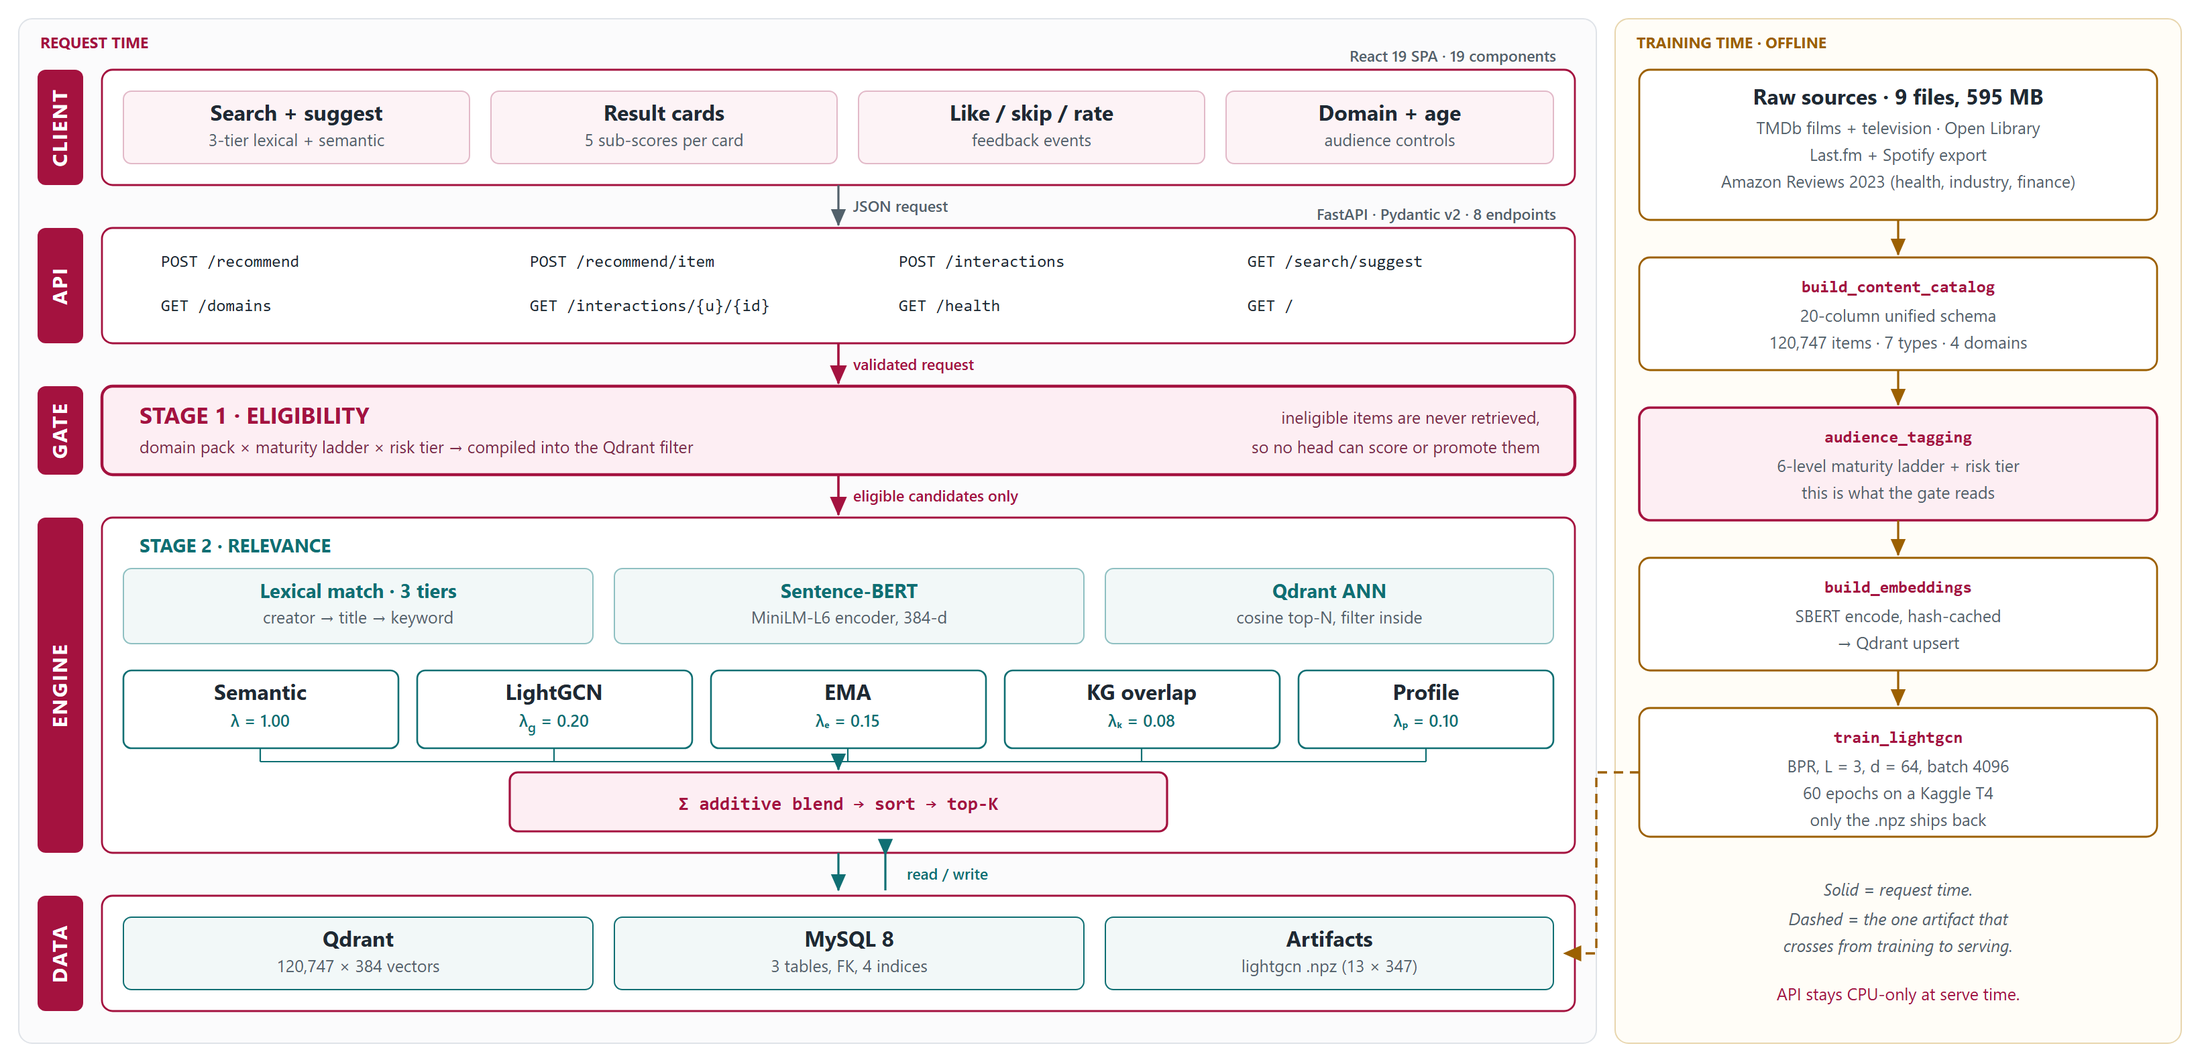
\includegraphics[width=\linewidth,height=6.3cm,keepaspectratio]{architecture}
\end{center}
\vspace{1mm}
{\scriptsize\textbf{The ordering is the design.}
\textcolor{amritaMaroon}{\textbf{Stage 1}} is a hard predicate --- it decides what may be retrieved
\emph{at all}, and is compiled into the vector query, so an ineligible item is never scored and no
head can promote it back. \textcolor{amritaTeal}{\textbf{Stage 2}} then ranks only what survived:
$S = S_{sem} + \lambda_g S_{graph} + \lambda_e S_{ema} + \lambda_k S_{kg} + \lambda_p S_{profile}$,
with every sub-score returned to the UI. The single dashed edge is the only thing that crosses from
training to serving --- one \texttt{.npz} file --- which is why the API stays CPU-only.}
\end{frame}

% ---------------------------------------------------------------------
\begin{frame}[fragile]{1. Modules, API Contract \& Database Schema}
\framesubtitle{Modular breakdown $\cdot$ REST contract $\cdot$ relational schema $\cdot$ deployment}
\vspace{0.5mm}
\begin{columns}[T]
\column{0.46\textwidth}
\blk{Module breakdown}
{\tiny
\renewcommand{\arraystretch}{1.34}
\begin{tabular}{p{1.5cm} p{2.3cm} p{1.95cm}}
\toprule
\textbf{Module} & \textbf{Responsibility} & \textbf{Location}\\
\midrule
Data layer      & Mapping, cleaning, catalog build & \texttt{preprocessing/}\\
Domain registry & Packs, risk tiers, advisories    & \texttt{domains.py}\\
Embedding       & SBERT encode, hash cache         & \texttt{embeddings/}\\
Retrieval       & ANN search, 3-tier lexical       & \texttt{qdrant\_rec.py}\\
Audience        & Eligibility filter, maturity     & \texttt{audience.py}\\
Adaptation      & EMA vector update, scoring       & \texttt{ema\_rec.py}\\
Graph CF        & LightGCN train, export, rerank   & \texttt{models/graph/}\\
Knowledge graph & Token overlap, profile scoring   & \texttt{knowledge\_g.py}\\
Persistence     & Catalog, profiles, events        & \texttt{mysql\_store.py}\\
API + UI        & Validation, DI, React SPA        & \texttt{app.py}\\
\bottomrule
\end{tabular}}

\column{0.515\textwidth}
\blk{Representative API contract}
{\tiny
\begin{verbatim}
POST /recommend
{ "query":"space adventure", "user_id":"u1",
  "domain":"entertainment", "age":15 }
-->
{ "advisory": null,
  "results":[ { "global_id","title","score",
    "semantic_score","graph_score","ema_score",
    "kg_score","profile_score","maturity",
    "match_kind","match_tier" } ] }
\end{verbatim}}
\vspace{-2mm}
\blk{Schema (MySQL 8)}
\vspace{-2mm}
\begin{itemize}\tiny\setlength{\itemsep}{2.5pt}
  \item \texttt{content\_entities}(\underline{global\_id}, content\_type, domain, maturity, audience\_min\_age, risk\_tier, title, creators, rating)
  \item \texttt{user\_profiles}(\underline{user\_id}, age\_group, profession, ema\_vector)
  \item \texttt{user\_interactions}(\underline{id}, user\_id, entity\_id FK, event\_type, timestamp) --- \textit{idx} \texttt{(user\_id, timestamp)}
\end{itemize}
\vspace{1mm}
{\tiny\textbf{Deployment.} Qdrant in Docker; MySQL 8; Uvicorn workers; Vite static build, same
origin. GPU training on Kaggle T4 --- only the \texttt{.npz} ships back, so the API is CPU-only.}
\end{columns}
\end{frame}

% =====================================================================
% RETRIEVAL & KNOWLEDGE GRAPH
% =====================================================================
\section{Retrieval \& Knowledge Graph}

\begin{frame}[shrink=15]{2. Data Layer --- Sources and Scale on Disk}
\framesubtitle{Rubric: Implementation Progress (8 Marks) $\cdot$ how large the data actually is}
\vspace{0.5mm}
\begin{columns}[T]
\column{0.535\textwidth}
\blk{Catalog composition --- 120{,}747 items}
{\tiny
\renewcommand{\arraystretch}{1.36}
\begin{tabular}{p{1.5cm} p{2.45cm} r}
\toprule
\textbf{Domain} & \textbf{Source} & \textbf{Items}\\
\midrule
Entertainment & TMDb films            & 23{,}492\\
Entertainment & TMDb television       & 10{,}617\\
Entertainment & Open Library books    & 12{,}402\\
Entertainment & Spotify data, Last.fm & 31{,}133\\
Health        & Amazon Reviews 2023   & 20{,}000\\
Industry      & Amazon Reviews 2023   & 20{,}000\\
Finance       & Amazon, Open Library  &  3{,}103\\
\midrule
\textbf{Total} & \textbf{9 source files} & \textbf{120{,}747}\\
\bottomrule
\end{tabular}}

\column{0.435\textwidth}
\blk{Disk footprint}
{\tiny
\renewcommand{\arraystretch}{1.40}
\begin{tabular}{p{3.5cm} r}
\toprule
Raw source datasets            & 595\,MB\\
Built catalog (20 columns)     & 277\,MB\\
Embedding matrix + index       & 379\,MB\\
Qdrant collection              & 605\,MB\\
\midrule
\textbf{Total working set}     & \textbf{$\approx$1.8\,GB}\\
\bottomrule
\end{tabular}}\\[2mm]
{\tiny The \emph{benchmark} data is larger again: Amazon Reviews 2023 supplies \textbf{7.4\,M} raw
interactions for Movies \& TV and \textbf{413\,k} for Industrial, streamed on Kaggle rather than
stored locally.}
\end{columns}
\vspace{2mm}
{\scriptsize\textbf{Why the Spotify API is not called.} Our music rows \emph{are} a Spotify export,
so the track ids are already correct and \texttt{/v1/tracks} would cover the catalog in
$\approx$570 requests. The blocker is on Spotify's side: client credentials authenticate
(token \texttt{200}), then every Web API endpoint returns \texttt{403 --- "Active premium
subscription required for the owner of the app"}. There is no free tier for this any more, so we
use \textbf{Last.fm} (free key) for volume and \textbf{iTunes Search} (no key) for coverage.
Only the artwork URL is read; it reaches no model.}
\end{frame}

% ---------------------------------------------------------------------
\begin{frame}{2. Retrieval --- Hybrid Lexical and Semantic}
\framesubtitle{Candidate generation: dense vectors for meaning, a lexical path for exact names}
\vspace{2mm}
\begin{columns}[T]
\column{0.485\textwidth}
\blk{Why one path was not enough}
\begin{itemize}\small\setlength{\itemsep}{5pt}
  \item Dense retrieval \emph{smears} exact names: the vector for "James Cameron" sits near every
        other director, so a name query returned topically similar films rather than his.
  \item The lexical path was restored \emph{beside} the vector path --- three tiers in order:
        \textbf{creator}, \textbf{title}, \textbf{keyword}.
  \item Lexical hits are capped at half the page, so an exact match never crowds out the semantic
        result set.
  \item Every result carries \texttt{match\_kind} and \texttt{match\_tier}, so the UI can show
        \emph{which field} matched.
\end{itemize}

\column{0.485\textwidth}
\blk{Trade-offs}
\begin{itemize}\small\setlength{\itemsep}{5pt}
  \item \textbf{Qdrant over FAISS.} Payload filtering happens \emph{inside} the ANN search. With
        FAISS the audience filter would have been a post-filter --- a correctness problem, not
        merely a slower path.
  \item \textbf{One 384-d space over per-domain models.} A finance book and a film are directly
        comparable, and adding a domain costs no retraining.
  \item \textbf{Reserved ranking slots.} Creator and title matches score above the cosine range
        ($1.2-0.1r$ and $1.30-0.06r$) so an exact name always wins. These are ranking slots by
        construction, not calibrated scores.
\end{itemize}
\end{columns}
\vfill
{\footnotesize $S_{\mathit{sem}} = \cos(\mathbf{e}_i, \mathbf{q})$ over one shared 384-d space for
queries, items and user vectors --- so cosine applies with no projection layer. \textbf{The limit of
this head:} semantic similarity cannot express \emph{behaviour}, which is exactly what the graph
model adds.}
\vfill
\end{frame}

% --- UI evidence (search.png / similar.png) --------------------------
% =====================================================================
%  UI EVIDENCE FRAMES  --  % =====================================================================
%  UI EVIDENCE FRAMES  --  % =====================================================================
%  UI EVIDENCE FRAMES  --  \input{frames_ui} from the main .tex
%
%  Images: search.png, similar.png -- captured from the running frontend
%  on 14 Sep 2026 (Vite dev server, profile "Sci-Fi Explorer", 1600x1000).
%  Every number quoted below is read off those two captures. If you
%  re-shoot the UI, re-read the numbers: they WILL change, and a panel
%  that checks a sub-score against the slide is the worst way to find out.
%
%  HEIGHT BUDGET: a 16:9 frame gives ~6.8cm of body. The screenshot
%  heights below are what keeps the bullets on the slide -- if you
%  enlarge an image, delete a bullet to pay for it.
% =====================================================================

% ---------------------------------------------------------------------
\begin{frame}[shrink=15]{2. System in Action --- Search and the Score Breakdown}
\framesubtitle{Every ranked card exposes the sub-scores that produced it}
\vspace{-1mm}
\begin{center}
\shot{search}{width=0.88\linewidth,height=4.3cm,keepaspectratio}%
{Search results with one card's score breakdown expanded.}
\end{center}
\vspace{-1.5mm}
\begin{columns}[T]
\column{0.485\textwidth}
\blk{What is on screen}
\begin{itemize}\tiny\setlength{\itemsep}{2.5pt}
  \item Query \texttt{"space adventure with aliens"} under the \texttt{Sci-Fi Explorer} profile ---
        \textbf{10 results in 3973\,ms}, spanning \textbf{movies and shows}.
  \item \textbf{\#1 Aliens in the Attic, 0.912.} The bars are the score, not decoration.
  \item The domain scope and viewer age travel as payload filters applied \emph{inside} the
        Qdrant search, not as a post-filter.
\end{itemize}

\column{0.485\textwidth}
\blk{The sub-scores sum to the printed total}
\begin{itemize}\tiny\setlength{\itemsep}{2.5pt}
  \item $0.681_{\mathit{sem}} + 0.100_{\mathit{profile}} + 0.090_{\mathit{ema}}
        + 0.040_{\mathit{kg}} = \mathbf{0.911}$, against a printed \textbf{0.912} --- the
        difference is rounding, and it is checkable on screen.
  \item \textcolor{amritaMaroon}{\textbf{Graph is struck through}} on this card: the item has no
        LightGCN embedding, so that head returns nothing and the other four still rank it.
        \textbf{Graceful degradation, live} --- not a slide claim.
\end{itemize}
\end{columns}
\end{frame}

% ---------------------------------------------------------------------
\begin{frame}[shrink=15]{2. System in Action --- Find Similar and the Feedback Loop}
\framesubtitle{Item-to-item retrieval through \texttt{POST /recommend/item} --- same heads, different anchor}
\vspace{0.5mm}
\begin{columns}[T]
\column{0.45\textwidth}
\vspace{-1mm}
\begin{center}
\shot{similar}{width=\linewidth,height=5.0cm,keepaspectratio}%
{The Find-similar drawer, anchored on a result card.}
\end{center}

\column{0.525\textwidth}
\blk{Same five heads, a different anchor}
\begin{itemize}\tiny\setlength{\itemsep}{2.5pt}
  \item The drawer calls \texttt{POST /recommend/item}: the query vector \emph{is} the anchor
        item's own 384-d embedding, so nothing is typed.
  \item \textbf{\#1 Minions \& Monsters, 0.847}
        $= 0.535_{\mathit{sem}} + 0.128_{\mathit{graph}} + 0.101_{\mathit{ema}}
        + 0.063_{\mathit{profile}} + 0.021_{\mathit{kg}}$.
  \item \textcolor{amritaMaroon}{\textbf{Graph contributes $+0.128$ here}}, where it was struck out
        on the previous slide. That is the \textbf{0.20\% artifact coverage} visible in the
        product: this anchor is in the trained artifact, the other was not.
  \item The \texttt{All ages} badge on the second card is the maturity label surfaced per result.
\end{itemize}
\vspace{1mm}
\blk{Closing the loop}
\begin{itemize}\tiny\setlength{\itemsep}{2.5pt}
  \item Any card's like / skip / rate $\rightarrow$ \texttt{POST /interactions} $\rightarrow$ MySQL
        $\rightarrow$ EMA update ($\alpha = 0.25$, \textbf{39\,$\mu$s}).
  \item The next query ranks from the updated vector --- one vector write, never a retrain.
\end{itemize}
\end{columns}
\end{frame}
 from the main .tex
%
%  Images: search.png, similar.png -- captured from the running frontend
%  on 14 Sep 2026 (Vite dev server, profile "Sci-Fi Explorer", 1600x1000).
%  Every number quoted below is read off those two captures. If you
%  re-shoot the UI, re-read the numbers: they WILL change, and a panel
%  that checks a sub-score against the slide is the worst way to find out.
%
%  HEIGHT BUDGET: a 16:9 frame gives ~6.8cm of body. The screenshot
%  heights below are what keeps the bullets on the slide -- if you
%  enlarge an image, delete a bullet to pay for it.
% =====================================================================

% ---------------------------------------------------------------------
\begin{frame}[shrink=15]{2. System in Action --- Search and the Score Breakdown}
\framesubtitle{Every ranked card exposes the sub-scores that produced it}
\vspace{-1mm}
\begin{center}
\shot{search}{width=0.88\linewidth,height=4.3cm,keepaspectratio}%
{Search results with one card's score breakdown expanded.}
\end{center}
\vspace{-1.5mm}
\begin{columns}[T]
\column{0.485\textwidth}
\blk{What is on screen}
\begin{itemize}\tiny\setlength{\itemsep}{2.5pt}
  \item Query \texttt{"space adventure with aliens"} under the \texttt{Sci-Fi Explorer} profile ---
        \textbf{10 results in 3973\,ms}, spanning \textbf{movies and shows}.
  \item \textbf{\#1 Aliens in the Attic, 0.912.} The bars are the score, not decoration.
  \item The domain scope and viewer age travel as payload filters applied \emph{inside} the
        Qdrant search, not as a post-filter.
\end{itemize}

\column{0.485\textwidth}
\blk{The sub-scores sum to the printed total}
\begin{itemize}\tiny\setlength{\itemsep}{2.5pt}
  \item $0.681_{\mathit{sem}} + 0.100_{\mathit{profile}} + 0.090_{\mathit{ema}}
        + 0.040_{\mathit{kg}} = \mathbf{0.911}$, against a printed \textbf{0.912} --- the
        difference is rounding, and it is checkable on screen.
  \item \textcolor{amritaMaroon}{\textbf{Graph is struck through}} on this card: the item has no
        LightGCN embedding, so that head returns nothing and the other four still rank it.
        \textbf{Graceful degradation, live} --- not a slide claim.
\end{itemize}
\end{columns}
\end{frame}

% ---------------------------------------------------------------------
\begin{frame}[shrink=15]{2. System in Action --- Find Similar and the Feedback Loop}
\framesubtitle{Item-to-item retrieval through \texttt{POST /recommend/item} --- same heads, different anchor}
\vspace{0.5mm}
\begin{columns}[T]
\column{0.45\textwidth}
\vspace{-1mm}
\begin{center}
\shot{similar}{width=\linewidth,height=5.0cm,keepaspectratio}%
{The Find-similar drawer, anchored on a result card.}
\end{center}

\column{0.525\textwidth}
\blk{Same five heads, a different anchor}
\begin{itemize}\tiny\setlength{\itemsep}{2.5pt}
  \item The drawer calls \texttt{POST /recommend/item}: the query vector \emph{is} the anchor
        item's own 384-d embedding, so nothing is typed.
  \item \textbf{\#1 Minions \& Monsters, 0.847}
        $= 0.535_{\mathit{sem}} + 0.128_{\mathit{graph}} + 0.101_{\mathit{ema}}
        + 0.063_{\mathit{profile}} + 0.021_{\mathit{kg}}$.
  \item \textcolor{amritaMaroon}{\textbf{Graph contributes $+0.128$ here}}, where it was struck out
        on the previous slide. That is the \textbf{0.20\% artifact coverage} visible in the
        product: this anchor is in the trained artifact, the other was not.
  \item The \texttt{All ages} badge on the second card is the maturity label surfaced per result.
\end{itemize}
\vspace{1mm}
\blk{Closing the loop}
\begin{itemize}\tiny\setlength{\itemsep}{2.5pt}
  \item Any card's like / skip / rate $\rightarrow$ \texttt{POST /interactions} $\rightarrow$ MySQL
        $\rightarrow$ EMA update ($\alpha = 0.25$, \textbf{39\,$\mu$s}).
  \item The next query ranks from the updated vector --- one vector write, never a retrain.
\end{itemize}
\end{columns}
\end{frame}
 from the main .tex
%
%  Images: search.png, similar.png -- captured from the running frontend
%  on 14 Sep 2026 (Vite dev server, profile "Sci-Fi Explorer", 1600x1000).
%  Every number quoted below is read off those two captures. If you
%  re-shoot the UI, re-read the numbers: they WILL change, and a panel
%  that checks a sub-score against the slide is the worst way to find out.
%
%  HEIGHT BUDGET: a 16:9 frame gives ~6.8cm of body. The screenshot
%  heights below are what keeps the bullets on the slide -- if you
%  enlarge an image, delete a bullet to pay for it.
% =====================================================================

% ---------------------------------------------------------------------
\begin{frame}[shrink=15]{2. System in Action --- Search and the Score Breakdown}
\framesubtitle{Every ranked card exposes the sub-scores that produced it}
\vspace{-1mm}
\begin{center}
\shot{search}{width=0.88\linewidth,height=4.3cm,keepaspectratio}%
{Search results with one card's score breakdown expanded.}
\end{center}
\vspace{-1.5mm}
\begin{columns}[T]
\column{0.485\textwidth}
\blk{What is on screen}
\begin{itemize}\tiny\setlength{\itemsep}{2.5pt}
  \item Query \texttt{"space adventure with aliens"} under the \texttt{Sci-Fi Explorer} profile ---
        \textbf{10 results in 3973\,ms}, spanning \textbf{movies and shows}.
  \item \textbf{\#1 Aliens in the Attic, 0.912.} The bars are the score, not decoration.
  \item The domain scope and viewer age travel as payload filters applied \emph{inside} the
        Qdrant search, not as a post-filter.
\end{itemize}

\column{0.485\textwidth}
\blk{The sub-scores sum to the printed total}
\begin{itemize}\tiny\setlength{\itemsep}{2.5pt}
  \item $0.681_{\mathit{sem}} + 0.100_{\mathit{profile}} + 0.090_{\mathit{ema}}
        + 0.040_{\mathit{kg}} = \mathbf{0.911}$, against a printed \textbf{0.912} --- the
        difference is rounding, and it is checkable on screen.
  \item \textcolor{amritaMaroon}{\textbf{Graph is struck through}} on this card: the item has no
        LightGCN embedding, so that head returns nothing and the other four still rank it.
        \textbf{Graceful degradation, live} --- not a slide claim.
\end{itemize}
\end{columns}
\end{frame}

% ---------------------------------------------------------------------
\begin{frame}[shrink=15]{2. System in Action --- Find Similar and the Feedback Loop}
\framesubtitle{Item-to-item retrieval through \texttt{POST /recommend/item} --- same heads, different anchor}
\vspace{0.5mm}
\begin{columns}[T]
\column{0.45\textwidth}
\vspace{-1mm}
\begin{center}
\shot{similar}{width=\linewidth,height=5.0cm,keepaspectratio}%
{The Find-similar drawer, anchored on a result card.}
\end{center}

\column{0.525\textwidth}
\blk{Same five heads, a different anchor}
\begin{itemize}\tiny\setlength{\itemsep}{2.5pt}
  \item The drawer calls \texttt{POST /recommend/item}: the query vector \emph{is} the anchor
        item's own 384-d embedding, so nothing is typed.
  \item \textbf{\#1 Minions \& Monsters, 0.847}
        $= 0.535_{\mathit{sem}} + 0.128_{\mathit{graph}} + 0.101_{\mathit{ema}}
        + 0.063_{\mathit{profile}} + 0.021_{\mathit{kg}}$.
  \item \textcolor{amritaMaroon}{\textbf{Graph contributes $+0.128$ here}}, where it was struck out
        on the previous slide. That is the \textbf{0.20\% artifact coverage} visible in the
        product: this anchor is in the trained artifact, the other was not.
  \item The \texttt{All ages} badge on the second card is the maturity label surfaced per result.
\end{itemize}
\vspace{1mm}
\blk{Closing the loop}
\begin{itemize}\tiny\setlength{\itemsep}{2.5pt}
  \item Any card's like / skip / rate $\rightarrow$ \texttt{POST /interactions} $\rightarrow$ MySQL
        $\rightarrow$ EMA update ($\alpha = 0.25$, \textbf{39\,$\mu$s}).
  \item The next query ranks from the updated vector --- one vector write, never a retrain.
\end{itemize}
\end{columns}
\end{frame}


% =====================================================================
% ===== SPEAKER BLOCK: Sanjay A. K. -- model design and evaluation
% =====================================================================
\section{Learning to Rank \& Evaluation}

\begin{frame}{2. Model Design --- Multi-Signal Ranking Pipeline}
\framesubtitle{One query becomes an explainable ranked list spanning four domains}
\vspace{1mm}
\begin{center}
  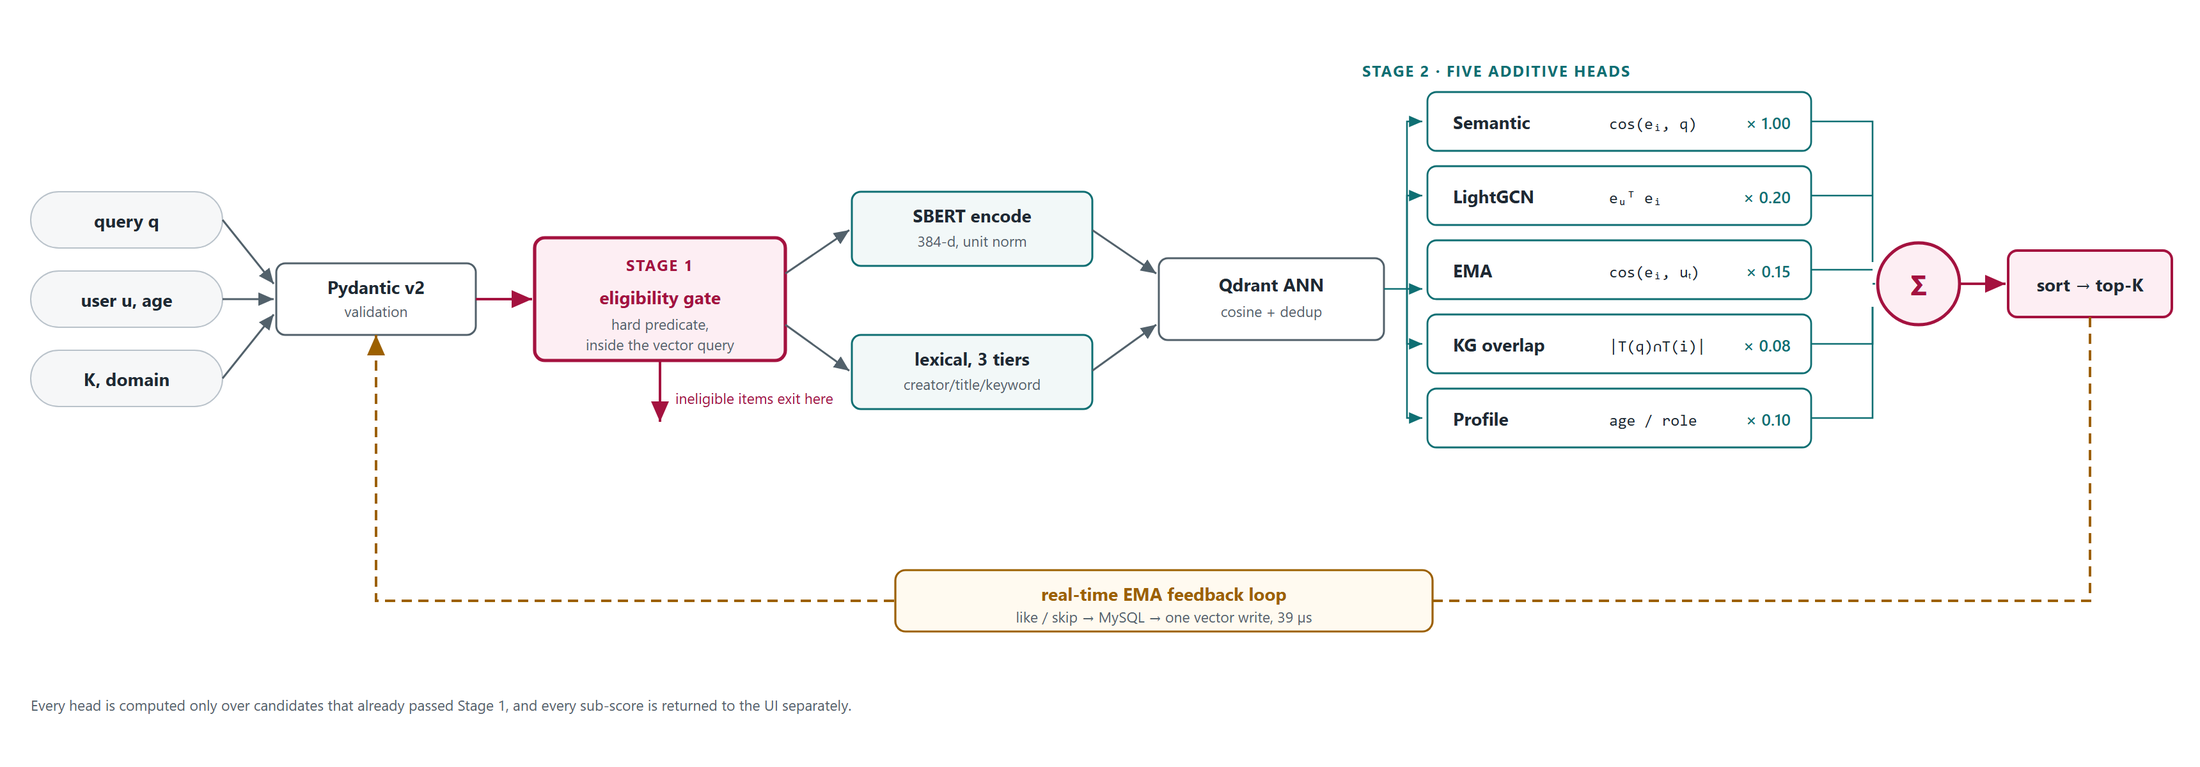
\includegraphics[width=\linewidth,height=5.4cm,keepaspectratio]{pipeline}
\end{center}

\vspace{2mm}
{\scriptsize\textbf{Reading the diagram.} The \textcolor{amritaMaroon}{\textbf{eligibility gate}} runs \emph{before} any head, so an ineligible item is never scored. The five heads then
run in parallel over the surviving candidates and are summed. Each head is defined on its own
slide --- algorithm, equation and measured result.}
\end{frame}

% --- model cards: one per model, algorithm + equation + diagram + metrics ---
% =====================================================================
%  MODEL CARDS  --  % =====================================================================
%  MODEL CARDS  --  % =====================================================================
%  MODEL CARDS  --  \input{models_frames} from 2_presentation.tex
%
%  Every card carries the same four things in the same order:
%     ALGORITHM  --  what it is, by name
%     EQUATION   --  what the code computes
%     DIAGRAM    --  the mechanism, drawn
%     MEASURED   --  a number from this repository
%
%  HEIGHT BUDGET -- READ THIS BEFORE ADDING A LINE.
%  A 16:9 frame gives ~6.8cm of body once title, subtitle and footline
%  are paid for. That is about 20 lines at \scriptsize, 27 at \tiny.
%  A display equation \[..\] costs ~3 lines.
%
%  Every card carries [shrink=15]: beamer measures the frame and scales
%  it down ONLY if it would overflow, up to 15%. A frame that already
%  fits is untouched. This is a SAFETY NET, not a licence to overfill --
%  past 15% the content runs off the bottom edge silently, exactly as it
%  did before. If you add an equation, delete a bullet to pay for it.
%
%  Overleaf prints "Overfull \vbox" for any frame that needed shrinking;
%  that warning is the signal to cut a line, not to raise the 15%.
%
%  All figures measured from the repository, 14 Sep 2026.
% =====================================================================

% ---------------------------------------------------------------------
\begin{frame}[shrink=15]{2. Model Inventory --- Five Scoring Heads and One Gate}
\framesubtitle{Each is a different model class, defined where the others are not}
\vspace{1mm}
\begin{center}
{\scriptsize
\renewcommand{\arraystretch}{1.22}
\begin{tabular}{c L{2.5cm} L{3.9cm} c c c}
\toprule
\textbf{Head} & \textbf{Model class} & \textbf{What it computes} & \textbf{Range} & \textbf{Cov.} & \textbf{Wt.}\\
\midrule
$S_{\mathit{sem}}$     & Transformer encoder   & Cosine to a 384-d sentence embedding & $[-1,1]$ & \textbf{100\%} & $1.00$\\
$S_{\mathit{graph}}$   & Graph neural net (CF) & Inner product of LightGCN embeddings & $[-1,1]$ & \textcolor{amritaMaroon}{\textbf{0.20\%}} & $0.20$\\
$S_{\mathit{ema}}$     & Online moving average & Cosine to the live user vector       & $[-1,1]$ & \textbf{100\%} & $0.15$\\
$S_{\mathit{kg}}$      & Set overlap, 0 params & Query / entity token overlap         & $[0,1]$  & \textbf{100\%} & $0.08$\\
$S_{\mathit{profile}}$ & Weighted term matcher & Declared-profile alignment           & $[-1,1]$ & \textbf{100\%} & $0.10$\\
\midrule
\textit{gate} & \textit{Hard predicate} & \textit{May this viewer see this item at all?} & $\{0,1\}$ & \textbf{100\%} & \textit{---}\\
\bottomrule
\end{tabular}}
\end{center}
\vspace{1mm}
{\scriptsize
\[ S(q,u,i) = S_{\mathit{sem}} + 0.20\,S_{\mathit{graph}} + 0.15\,S_{\mathit{ema}} + 0.08\,S_{\mathit{kg}} + 0.10\,S_{\mathit{profile}} \]}
\vspace{-3mm}
{\scriptsize\textbf{Why coverage is the column that matters.} The graph head is our strongest signal
and is defined for \textbf{0.20\%} of the catalog; every other head is defined everywhere. That is
why the blend is additive with a dominant semantic term rather than a learned gate --- a missing
head must degrade the ranking, never break it.}
\end{frame}

% ---------------------------------------------------------------------
\begin{frame}[shrink=15]{2. Model 1 --- SBERT Semantic Encoder}
\framesubtitle{Algorithm $\cdot$ equation $\cdot$ measured result}
\vspace{1mm}
\begin{center}
  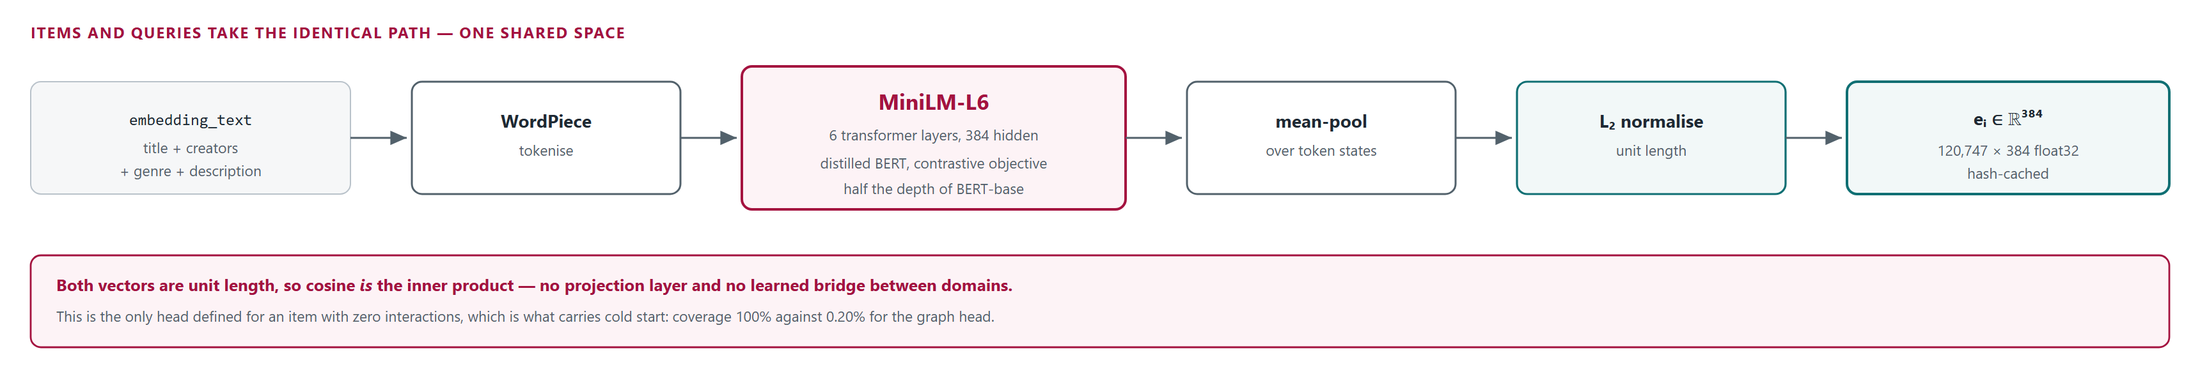
\includegraphics[width=\linewidth,height=3.4cm,keepaspectratio]{sbert}
\end{center}
\vspace{2mm}
\begin{columns}[T]
\column{0.485\textwidth}
\blk{Algorithm and equation}
{\scriptsize \texttt{all-MiniLM-L6-v2} --- a 6-layer distilled BERT, mean pooling over token states.
\[ \mathbf{e}_i = \frac{\mathrm{MeanPool}(\mathrm{MiniLM}(t_i))}{\lVert\cdot\rVert_2}, \quad
   S_{\mathit{sem}} = \mathbf{e}_i^{\top}\mathbf{q} \]
Both vectors are unit length, so cosine \emph{is} the inner product. The query takes the identical
path --- one shared space, no projection layer.}

\column{0.485\textwidth}
\blk{Measured}
\begin{tight}
  \item \textbf{120{,}747 $\times$ 384} float32; batch 256; hash-cached, so only changed rows
        re-encode.
  \item \textbf{Coverage 100\%} --- the only head defined at zero interactions, which is what
        carries cold start.
  \item 6 layers not 12, so the catalog encodes in one GPU pass and serving stays CPU-only.
\end{tight}
\end{columns}
\end{frame}

% ---------------------------------------------------------------------
\begin{frame}[shrink=15]{2. Model 2 --- LightGCN Graph Collaborative Filtering}
\framesubtitle{Algorithm $\cdot$ equation $\cdot$ measured result}
\vspace{1mm}
\begin{columns}[T]
\column{0.45\textwidth}
\blk{Algorithm}
{\scriptsize LightGCN (He et al., SIGIR 2020) --- a \emph{linear} convolution on the user--item
bipartite graph. Unlike NGCF there is \textbf{no feature transform and no nonlinearity}; the only
learned parameters are the layer-0 embeddings.}
\vspace{1.5mm}

\blk{Equations, as implemented}
{\scriptsize
With $\tilde{A} = D^{-1/2} A D^{-1/2}$, propagate and take the layer mean:
\[ \mathbf{E}^{(\ell)} = \tilde{A}\mathbf{E}^{(\ell-1)}, \quad
   \mathbf{E} = \tfrac{1}{L+1}\textstyle\sum_{\ell=0}^{L}\mathbf{E}^{(\ell)} \]
Score, and train by the BPR pairwise objective:
\[ \hat y_{ui} = \mathbf{e}_u^{\top}\mathbf{e}_i \]
\[ \mathcal{L} = -\!\sum \ln\sigma(\hat y_{ui}-\hat y_{uj}) + \lambda\lVert\mathbf{E}^{(0)}\rVert^2 \]}
\vspace{-1mm}
{\tiny\textbf{Config:} $d{=}64$, $L{=}3$, lr $10^{-3}$, decay $10^{-4}$, batch \textbf{4096},
60 epochs, seed 42, Kaggle T4.}

\column{0.52\textwidth}
\blk{Measured --- against a popularity control}
{\tiny
\renewcommand{\arraystretch}{1.15}
\begin{tabular}{L{1.4cm} l c c c c}
\toprule
\textbf{Domain} & \textbf{Model} & \textbf{R@20} & \textbf{N@20} & \textbf{MRR} & \textbf{Lift}\\
\midrule
Movies \& TV & LightGCN & \textbf{0.0288} & \textbf{0.0125} & \textbf{0.0080} & \\
             & popular  & 0.0182 & 0.0080 & 0.0052 & \textbf{1.59$\times$}\\
\midrule
Industrial   & LightGCN & \textbf{0.0326} & \textbf{0.0138} & \textbf{0.0087} & \\
             & popular  & 0.0264 & 0.0111 & 0.0070 & \textbf{1.24$\times$}\\
\midrule
Health       & LightGCN & 0.0121 & 0.0046 & 0.0025 & \\
             & popular  & \textbf{0.0221} & \textbf{0.0093} & \textbf{0.0059} & \textcolor{amritaMaroon}{\textbf{0.55$\times$}}\\
\bottomrule
\end{tabular}}\\[1.5mm]
{\tiny\textbf{Protocol.} Ratings $\geq 4$ as implicit positives; 10-core (Industrial keeps the
source 5-core floor); leave-last-out; 49{,}958 / 33{,}929 / 50{,}000 users evaluated.}\\[1.5mm]
{\tiny\textbf{$\mathtt{recall}=\mathtt{hit\_rate}$ is correct, not a bug:} leave-last-out gives one
relevant item, so Recall@$K \equiv$ HitRate@$K$. Check: $0.0288/20 = 0.00144$.}\\[1.5mm]
{\tiny\textcolor{amritaMaroon}{\textbf{Health regresses.}} BPR trains on the raw inner product, but
evaluation and serving both $L_2$-normalise and rank by cosine --- dividing by the \emph{item} norm
is not rank-preserving, and that norm carries the popularity prior.}
\end{columns}
\end{frame}

% ---------------------------------------------------------------------
%  PANEL RECOMMENDATION 1 -- NCF: position, architecture and plan
% ---------------------------------------------------------------------
\begin{frame}[shrink=15]{2. Panel Recommendation --- Neural Collaborative Filtering}
\framesubtitle{What NCF is, how it differs from LightGCN, and how we will test it}
\vspace{1mm}
\begin{columns}[T]
\column{0.475\textwidth}
\blk{What the panel asked for}
{\scriptsize NCF (He et al., WWW 2017) replaces the \emph{fixed} inner product with a \emph{learned}
similarity. NeuMF runs two towers and fuses them:
\[ \hat y^{\mathit{GMF}} = \mathbf{p}_u \odot \mathbf{q}_i, \quad
   \hat y^{\mathit{MLP}} = \phi_L(\cdots\phi_1([\mathbf{p}'_u \| \mathbf{q}'_i])) \]
\[ \hat y_{ui} = \sigma\big(\mathbf{h}^{\top}[\,\hat y^{\mathit{GMF}} \,\|\, \hat y^{\mathit{MLP}}\,]\big) \]
The MLP tower models \textbf{non-linear} interaction --- which our inner product cannot.}
\vspace{1.5mm}

\blk{How it differs from what we run}
\begin{tight}
  \item \textbf{LightGCN is graph-based:} it propagates over the bipartite graph, so a user is
        informed by items three hops away. \textbf{NCF has no graph} --- it learns a similarity on
        ids alone. They are complementary, not substitutes.
\end{tight}

\column{0.495\textwidth}
\vspace{-2mm}
\begin{center}
  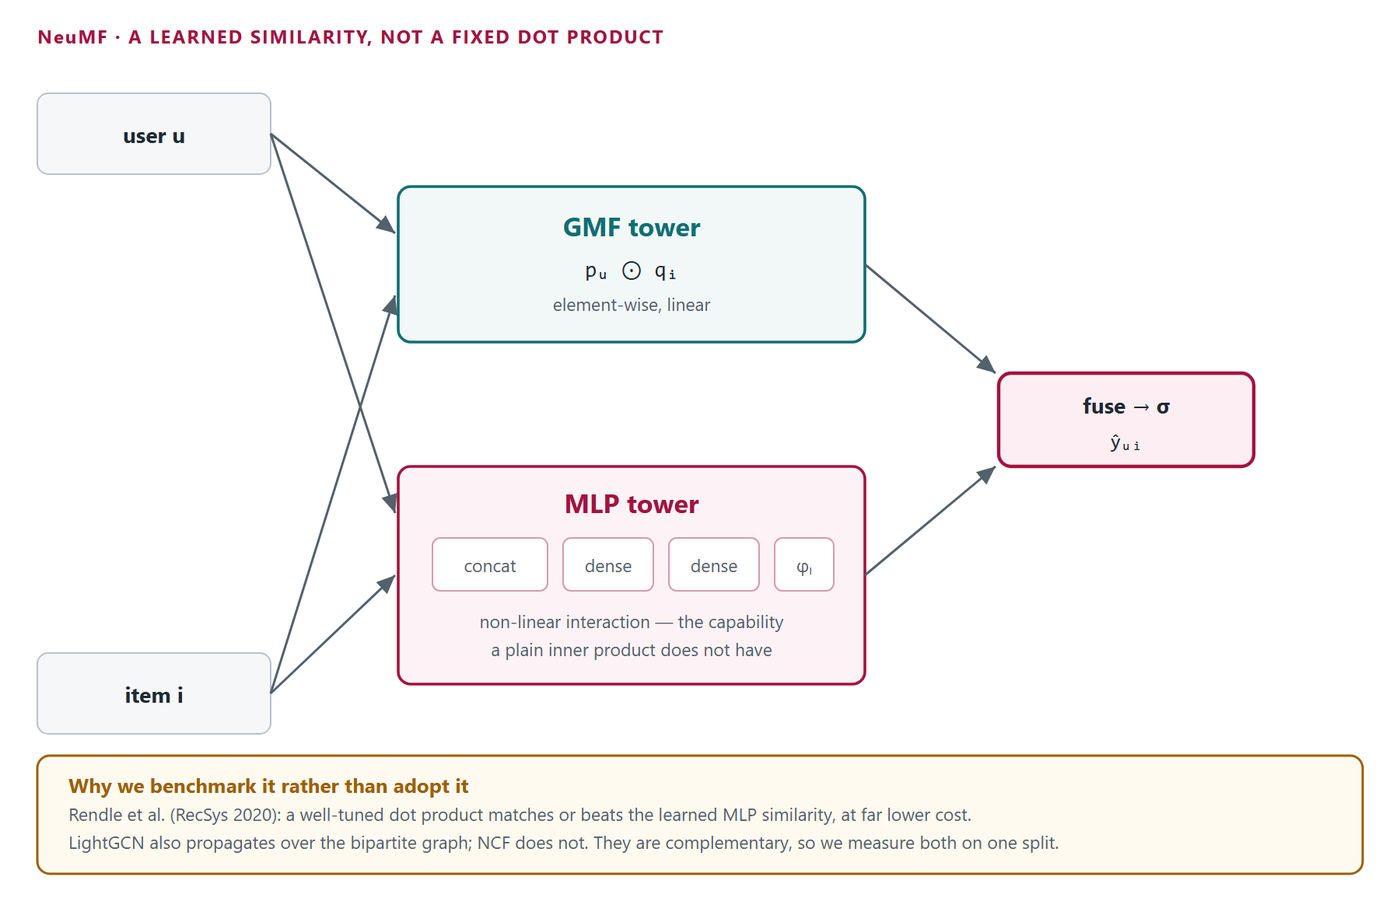
\includegraphics[width=\linewidth,height=4.9cm,keepaspectratio]{ncf}
\end{center}
\vspace{1mm}

\blk{Our position, and the plan}
\begin{tight}
  \item Rendle et al.\ (RecSys 2020) revisited this comparison and found a \textbf{well-tuned dot
        product matches or beats} the learned MLP, at far lower cost --- so we will run NeuMF as a
        \emph{measured baseline}, not adopt it as an assumed upgrade.
  \item The harness already runs three domains on fixed splits, so NeuMF slots in behind the same
        interface; then report popularity / LightGCN / NeuMF side by side.
\end{tight}
\end{columns}
\end{frame}

% ---------------------------------------------------------------------
\begin{frame}[shrink=15]{2. Model 3 --- Real-Time EMA User Vector}
\framesubtitle{Algorithm $\cdot$ equation $\cdot$ measured result}
\vspace{1mm}
\begin{columns}[T]
\column{0.515\textwidth}
\blk{Algorithm}
{\scriptsize A \textbf{signed, strength-scaled} exponential moving average in the same 384-d space
as the items. Not a plain average: a negative event pushes the user vector \emph{away} from the
item, and the step scales with how strong the event was.}
\vspace{1.5mm}

\blk{Equations, as implemented}
{\scriptsize
Event weight $w$: $+1.2$ complete, $+1.0$ like, $+0.6$ click, $+0.4$ view, $-1.0$ skip; a rating
$v$ maps to $(v-3)/2$. Then with $\alpha = 0.25$:
\[ d=\operatorname{sign}(w),\ \ s=\min(|w|,1),\ \ \eta=\operatorname{clip}(\alpha s,0,1) \]
\[ \mathbf{u}_{t+1} = \frac{(1-\eta)\mathbf{u}_t + \eta\,d\,\mathbf{e}_i}{\lVert\cdot\rVert_2},
   \ \ S_{\mathit{ema}} = \mathbf{u}_t^{\top}\mathbf{e}_i \]}

\column{0.46\textwidth}
\vspace{-3mm}
\begin{center}
  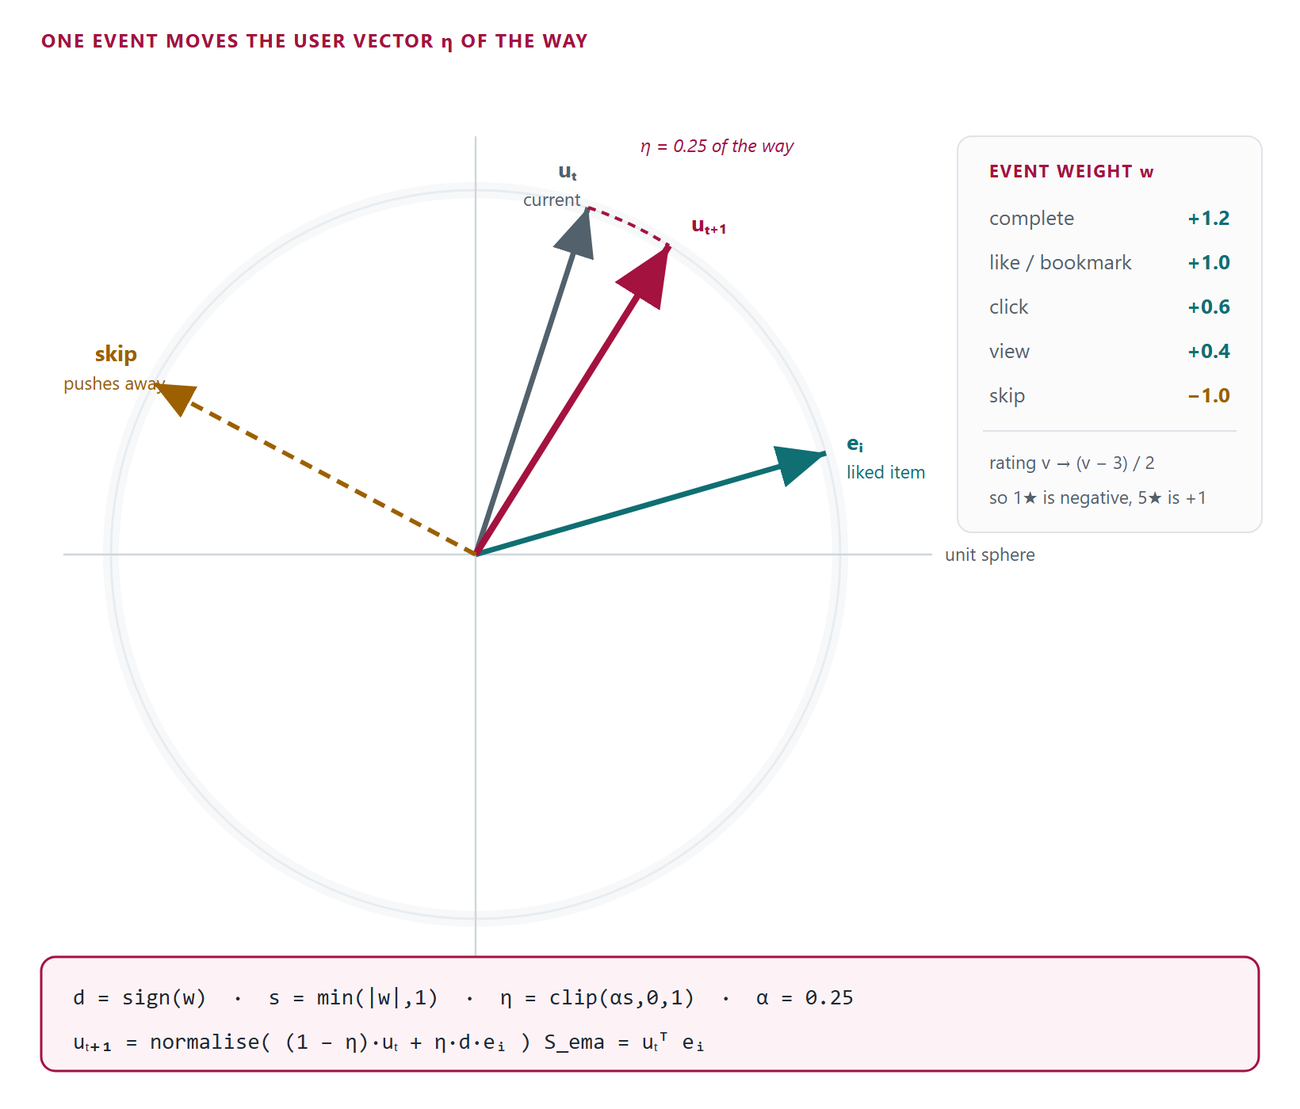
\includegraphics[width=\linewidth,height=5.5cm,keepaspectratio]{ema}
\end{center}
\vspace{1mm}

\blk{Measured}
\begin{tight}
  \item \textbf{39.0\,$\mu$s} per update, \textbf{16.7\,$\mu$s} per score (1{,}000 ops, 384-d).
  \item Against \textbf{hours} for a retrain --- five orders of magnitude. This is the "real-time"
        in the project title, as a number.
  \item \textbf{Limitation:} no session boundary or time decay, so one misclick persists.
\end{tight}
\end{columns}
\end{frame}

% ---------------------------------------------------------------------
\begin{frame}[shrink=15]{2. Model 4 --- Knowledge-Graph Overlap Head}
\framesubtitle{Algorithm $\cdot$ equation $\cdot$ measured result}
\vspace{1mm}
\begin{columns}[T]
\column{0.47\textwidth}
\blk{Algorithm and equation}
{\scriptsize A \textbf{zero-parameter set-overlap scorer} over shared entity namespaces. Nothing is
trained, so nothing drifts --- and it is defined precisely where the graph model is not. With
$T(i)$ the token set over \{title, description, creators, categories, type\}:
\[ S_{\mathit{kg}} = \min\!\left(1,\ \frac{|T(q)\cap T(i)|}{\max(3,|T(q)|)}\right) \]
The $\max(3,\cdot)$ floor stops a one-word query scoring 1.0 on one incidental match.}
\vspace{1.5mm}

\blk{Measured}
\begin{tight}
  \item Mean \textbf{KG@5 $=$ 0.892} over 8 scenarios; \textbf{0.667} on both named-entity queries,
        where dense retrieval smears.
  \item \textbf{Coverage 100\%} --- it reads metadata, not behaviour.
\end{tight}

\column{0.50\textwidth}
\vspace{-3mm}
\begin{center}
  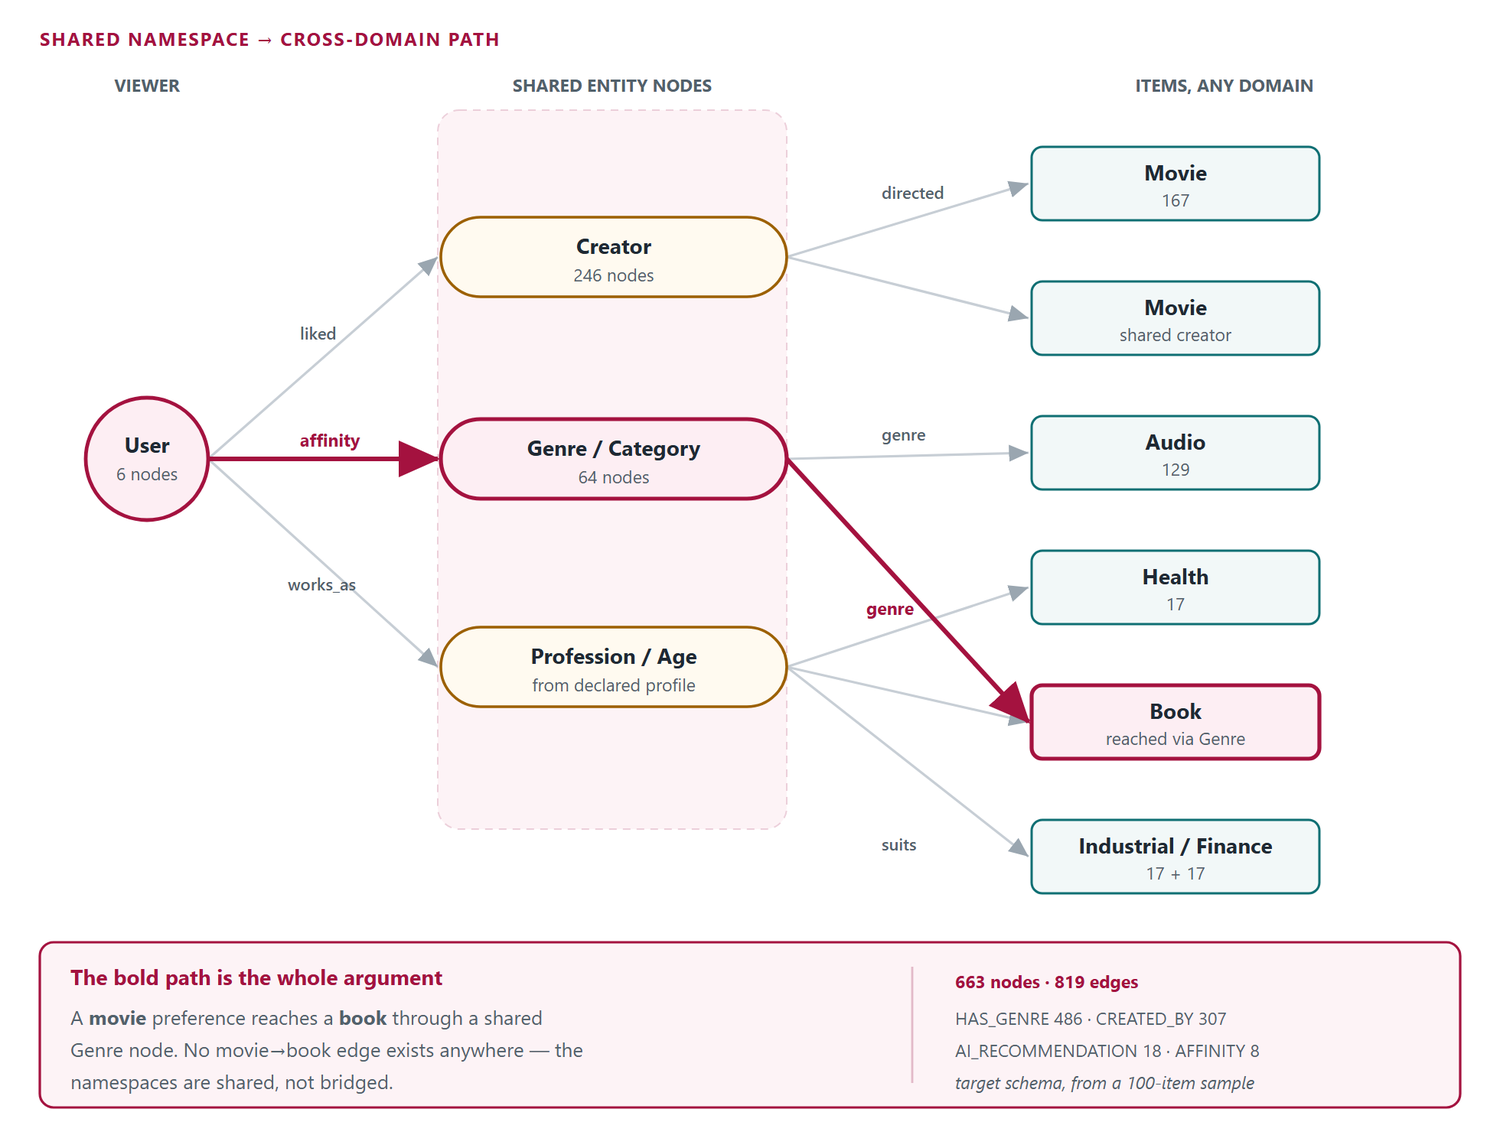
\includegraphics[width=\linewidth,height=5.7cm,keepaspectratio]{kg}
\end{center}
\vspace{1mm}

{\scriptsize\textcolor{amritaMaroon}{\textbf{Bold path:}} a \emph{movie} preference reaches a
\emph{book} through a shared Genre node --- no movie-to-book edge exists anywhere.}\\[1mm]
{\tiny\textbf{Scope.} At request time this is the overlap function above; the 663-node figure is the
\emph{target schema} from a 100-item example, not a runtime graph. Neo4j is Review 3.}
\end{columns}
\end{frame}

% ---------------------------------------------------------------------
\begin{frame}[shrink=15]{2. Model 5 --- Profile Head and the Eligibility Gate}
\framesubtitle{Algorithm $\cdot$ equation $\cdot$ measured result}
\vspace{1mm}
\begin{columns}[T]
\column{0.53\textwidth}
\blk{Profile head --- a score}
{\footnotesize A \textbf{weighted term matcher} against the declared profile; avoid-terms subtract
at nearly twice the weight of a positive match.
\[ S_{\mathit{profile}} = \operatorname{clip}\big(0.16|P\cap i| - 0.25|A\cap i| + 0.15\cdot\mathbf{1}[\tau_i \in \Pi]\big) \]}
\vspace{-3mm}
{\scriptsize $P$ = interests $\cup$ likes $\cup$ skills $\cup$ role $\cup$ age terms; \ $A$ = avoid
terms; \ $\Pi$ = preferred types; clipped to $[-1,1]$.}
\vspace{3mm}

\blk{Eligibility --- a predicate, not a score}
{\footnotesize
\[ \mathrm{elig}(i\,|\,c) = \mathbf{1}\big[a_{\mathit{eff}} \geq \mathrm{minage}(i)\big] \wedge \mathbf{1}\big[\tau_i \in \mathcal{T}(d)\big] \]
Compiled \emph{into} the Qdrant query, so an ineligible item is never retrieved, never scored, and
cannot be promoted back by any head.}
\vspace{2mm}

{\footnotesize\textbf{Fail-closed.} No age supplied caps at teen, not adult. Unknown metadata falls
back to the content-type default, never to unrestricted. Health and finance are \textbf{discovery
only, never advice}.}

\column{0.445\textwidth}
\vspace{-2mm}
\begin{center}
  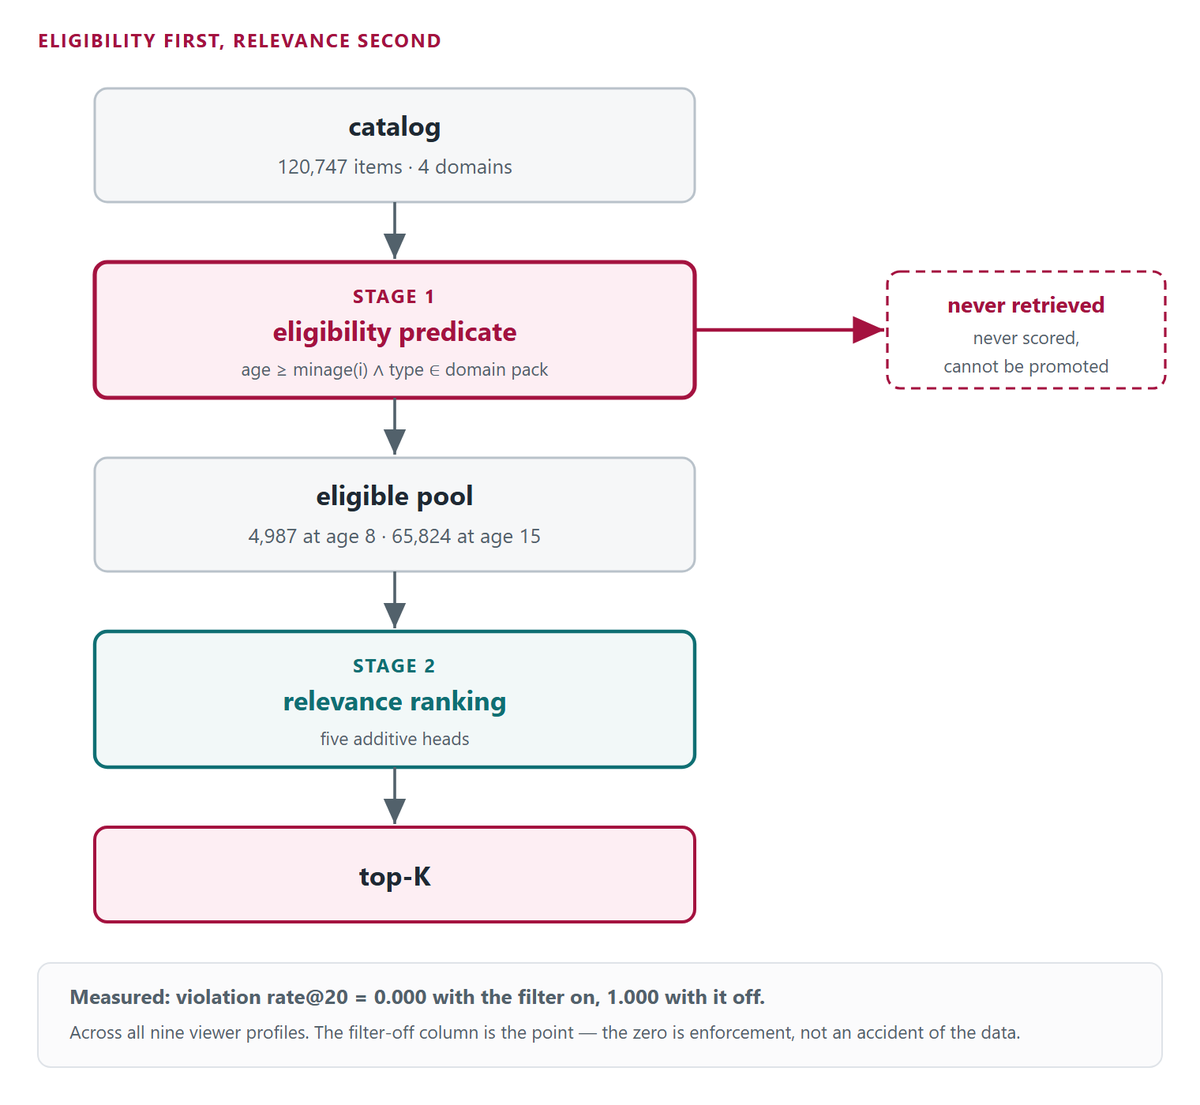
\includegraphics[width=\linewidth,height=5.9cm,keepaspectratio]{gate}
\end{center}
\vspace{2mm}
\blk{Measured}
\begin{tight}
  \item Mean \textbf{profile@5 $=$ 0.957}; \textbf{8 of 8} scenarios fully profile-positive.
  \item Violations \textbf{0.000} on, \textbf{1.000} off, across \textbf{9} viewer profiles.
\end{tight}
\end{columns}
\end{frame}
 from 2_presentation.tex
%
%  Every card carries the same four things in the same order:
%     ALGORITHM  --  what it is, by name
%     EQUATION   --  what the code computes
%     DIAGRAM    --  the mechanism, drawn
%     MEASURED   --  a number from this repository
%
%  HEIGHT BUDGET -- READ THIS BEFORE ADDING A LINE.
%  A 16:9 frame gives ~6.8cm of body once title, subtitle and footline
%  are paid for. That is about 20 lines at \scriptsize, 27 at \tiny.
%  A display equation \[..\] costs ~3 lines.
%
%  Every card carries [shrink=15]: beamer measures the frame and scales
%  it down ONLY if it would overflow, up to 15%. A frame that already
%  fits is untouched. This is a SAFETY NET, not a licence to overfill --
%  past 15% the content runs off the bottom edge silently, exactly as it
%  did before. If you add an equation, delete a bullet to pay for it.
%
%  Overleaf prints "Overfull \vbox" for any frame that needed shrinking;
%  that warning is the signal to cut a line, not to raise the 15%.
%
%  All figures measured from the repository, 14 Sep 2026.
% =====================================================================

% ---------------------------------------------------------------------
\begin{frame}[shrink=15]{2. Model Inventory --- Five Scoring Heads and One Gate}
\framesubtitle{Each is a different model class, defined where the others are not}
\vspace{1mm}
\begin{center}
{\scriptsize
\renewcommand{\arraystretch}{1.22}
\begin{tabular}{c L{2.5cm} L{3.9cm} c c c}
\toprule
\textbf{Head} & \textbf{Model class} & \textbf{What it computes} & \textbf{Range} & \textbf{Cov.} & \textbf{Wt.}\\
\midrule
$S_{\mathit{sem}}$     & Transformer encoder   & Cosine to a 384-d sentence embedding & $[-1,1]$ & \textbf{100\%} & $1.00$\\
$S_{\mathit{graph}}$   & Graph neural net (CF) & Inner product of LightGCN embeddings & $[-1,1]$ & \textcolor{amritaMaroon}{\textbf{0.20\%}} & $0.20$\\
$S_{\mathit{ema}}$     & Online moving average & Cosine to the live user vector       & $[-1,1]$ & \textbf{100\%} & $0.15$\\
$S_{\mathit{kg}}$      & Set overlap, 0 params & Query / entity token overlap         & $[0,1]$  & \textbf{100\%} & $0.08$\\
$S_{\mathit{profile}}$ & Weighted term matcher & Declared-profile alignment           & $[-1,1]$ & \textbf{100\%} & $0.10$\\
\midrule
\textit{gate} & \textit{Hard predicate} & \textit{May this viewer see this item at all?} & $\{0,1\}$ & \textbf{100\%} & \textit{---}\\
\bottomrule
\end{tabular}}
\end{center}
\vspace{1mm}
{\scriptsize
\[ S(q,u,i) = S_{\mathit{sem}} + 0.20\,S_{\mathit{graph}} + 0.15\,S_{\mathit{ema}} + 0.08\,S_{\mathit{kg}} + 0.10\,S_{\mathit{profile}} \]}
\vspace{-3mm}
{\scriptsize\textbf{Why coverage is the column that matters.} The graph head is our strongest signal
and is defined for \textbf{0.20\%} of the catalog; every other head is defined everywhere. That is
why the blend is additive with a dominant semantic term rather than a learned gate --- a missing
head must degrade the ranking, never break it.}
\end{frame}

% ---------------------------------------------------------------------
\begin{frame}[shrink=15]{2. Model 1 --- SBERT Semantic Encoder}
\framesubtitle{Algorithm $\cdot$ equation $\cdot$ measured result}
\vspace{1mm}
\begin{center}
  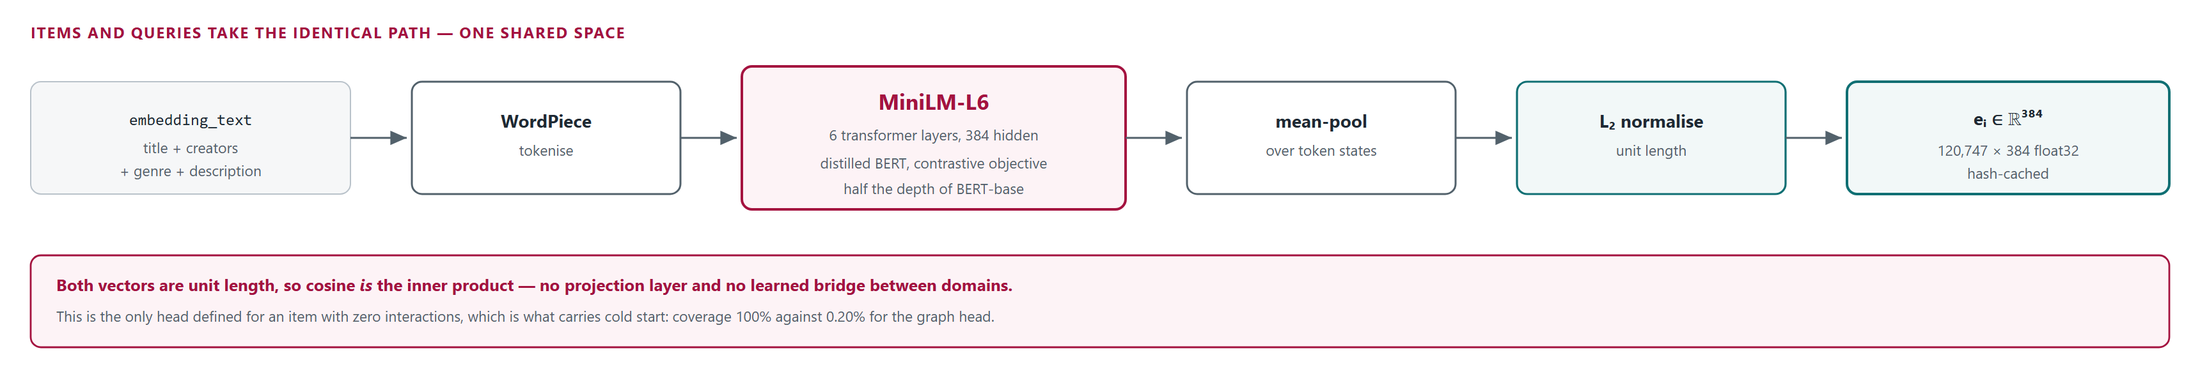
\includegraphics[width=\linewidth,height=3.4cm,keepaspectratio]{sbert}
\end{center}
\vspace{2mm}
\begin{columns}[T]
\column{0.485\textwidth}
\blk{Algorithm and equation}
{\scriptsize \texttt{all-MiniLM-L6-v2} --- a 6-layer distilled BERT, mean pooling over token states.
\[ \mathbf{e}_i = \frac{\mathrm{MeanPool}(\mathrm{MiniLM}(t_i))}{\lVert\cdot\rVert_2}, \quad
   S_{\mathit{sem}} = \mathbf{e}_i^{\top}\mathbf{q} \]
Both vectors are unit length, so cosine \emph{is} the inner product. The query takes the identical
path --- one shared space, no projection layer.}

\column{0.485\textwidth}
\blk{Measured}
\begin{tight}
  \item \textbf{120{,}747 $\times$ 384} float32; batch 256; hash-cached, so only changed rows
        re-encode.
  \item \textbf{Coverage 100\%} --- the only head defined at zero interactions, which is what
        carries cold start.
  \item 6 layers not 12, so the catalog encodes in one GPU pass and serving stays CPU-only.
\end{tight}
\end{columns}
\end{frame}

% ---------------------------------------------------------------------
\begin{frame}[shrink=15]{2. Model 2 --- LightGCN Graph Collaborative Filtering}
\framesubtitle{Algorithm $\cdot$ equation $\cdot$ measured result}
\vspace{1mm}
\begin{columns}[T]
\column{0.45\textwidth}
\blk{Algorithm}
{\scriptsize LightGCN (He et al., SIGIR 2020) --- a \emph{linear} convolution on the user--item
bipartite graph. Unlike NGCF there is \textbf{no feature transform and no nonlinearity}; the only
learned parameters are the layer-0 embeddings.}
\vspace{1.5mm}

\blk{Equations, as implemented}
{\scriptsize
With $\tilde{A} = D^{-1/2} A D^{-1/2}$, propagate and take the layer mean:
\[ \mathbf{E}^{(\ell)} = \tilde{A}\mathbf{E}^{(\ell-1)}, \quad
   \mathbf{E} = \tfrac{1}{L+1}\textstyle\sum_{\ell=0}^{L}\mathbf{E}^{(\ell)} \]
Score, and train by the BPR pairwise objective:
\[ \hat y_{ui} = \mathbf{e}_u^{\top}\mathbf{e}_i \]
\[ \mathcal{L} = -\!\sum \ln\sigma(\hat y_{ui}-\hat y_{uj}) + \lambda\lVert\mathbf{E}^{(0)}\rVert^2 \]}
\vspace{-1mm}
{\tiny\textbf{Config:} $d{=}64$, $L{=}3$, lr $10^{-3}$, decay $10^{-4}$, batch \textbf{4096},
60 epochs, seed 42, Kaggle T4.}

\column{0.52\textwidth}
\blk{Measured --- against a popularity control}
{\tiny
\renewcommand{\arraystretch}{1.15}
\begin{tabular}{L{1.4cm} l c c c c}
\toprule
\textbf{Domain} & \textbf{Model} & \textbf{R@20} & \textbf{N@20} & \textbf{MRR} & \textbf{Lift}\\
\midrule
Movies \& TV & LightGCN & \textbf{0.0288} & \textbf{0.0125} & \textbf{0.0080} & \\
             & popular  & 0.0182 & 0.0080 & 0.0052 & \textbf{1.59$\times$}\\
\midrule
Industrial   & LightGCN & \textbf{0.0326} & \textbf{0.0138} & \textbf{0.0087} & \\
             & popular  & 0.0264 & 0.0111 & 0.0070 & \textbf{1.24$\times$}\\
\midrule
Health       & LightGCN & 0.0121 & 0.0046 & 0.0025 & \\
             & popular  & \textbf{0.0221} & \textbf{0.0093} & \textbf{0.0059} & \textcolor{amritaMaroon}{\textbf{0.55$\times$}}\\
\bottomrule
\end{tabular}}\\[1.5mm]
{\tiny\textbf{Protocol.} Ratings $\geq 4$ as implicit positives; 10-core (Industrial keeps the
source 5-core floor); leave-last-out; 49{,}958 / 33{,}929 / 50{,}000 users evaluated.}\\[1.5mm]
{\tiny\textbf{$\mathtt{recall}=\mathtt{hit\_rate}$ is correct, not a bug:} leave-last-out gives one
relevant item, so Recall@$K \equiv$ HitRate@$K$. Check: $0.0288/20 = 0.00144$.}\\[1.5mm]
{\tiny\textcolor{amritaMaroon}{\textbf{Health regresses.}} BPR trains on the raw inner product, but
evaluation and serving both $L_2$-normalise and rank by cosine --- dividing by the \emph{item} norm
is not rank-preserving, and that norm carries the popularity prior.}
\end{columns}
\end{frame}

% ---------------------------------------------------------------------
%  PANEL RECOMMENDATION 1 -- NCF: position, architecture and plan
% ---------------------------------------------------------------------
\begin{frame}[shrink=15]{2. Panel Recommendation --- Neural Collaborative Filtering}
\framesubtitle{What NCF is, how it differs from LightGCN, and how we will test it}
\vspace{1mm}
\begin{columns}[T]
\column{0.475\textwidth}
\blk{What the panel asked for}
{\scriptsize NCF (He et al., WWW 2017) replaces the \emph{fixed} inner product with a \emph{learned}
similarity. NeuMF runs two towers and fuses them:
\[ \hat y^{\mathit{GMF}} = \mathbf{p}_u \odot \mathbf{q}_i, \quad
   \hat y^{\mathit{MLP}} = \phi_L(\cdots\phi_1([\mathbf{p}'_u \| \mathbf{q}'_i])) \]
\[ \hat y_{ui} = \sigma\big(\mathbf{h}^{\top}[\,\hat y^{\mathit{GMF}} \,\|\, \hat y^{\mathit{MLP}}\,]\big) \]
The MLP tower models \textbf{non-linear} interaction --- which our inner product cannot.}
\vspace{1.5mm}

\blk{How it differs from what we run}
\begin{tight}
  \item \textbf{LightGCN is graph-based:} it propagates over the bipartite graph, so a user is
        informed by items three hops away. \textbf{NCF has no graph} --- it learns a similarity on
        ids alone. They are complementary, not substitutes.
\end{tight}

\column{0.495\textwidth}
\vspace{-2mm}
\begin{center}
  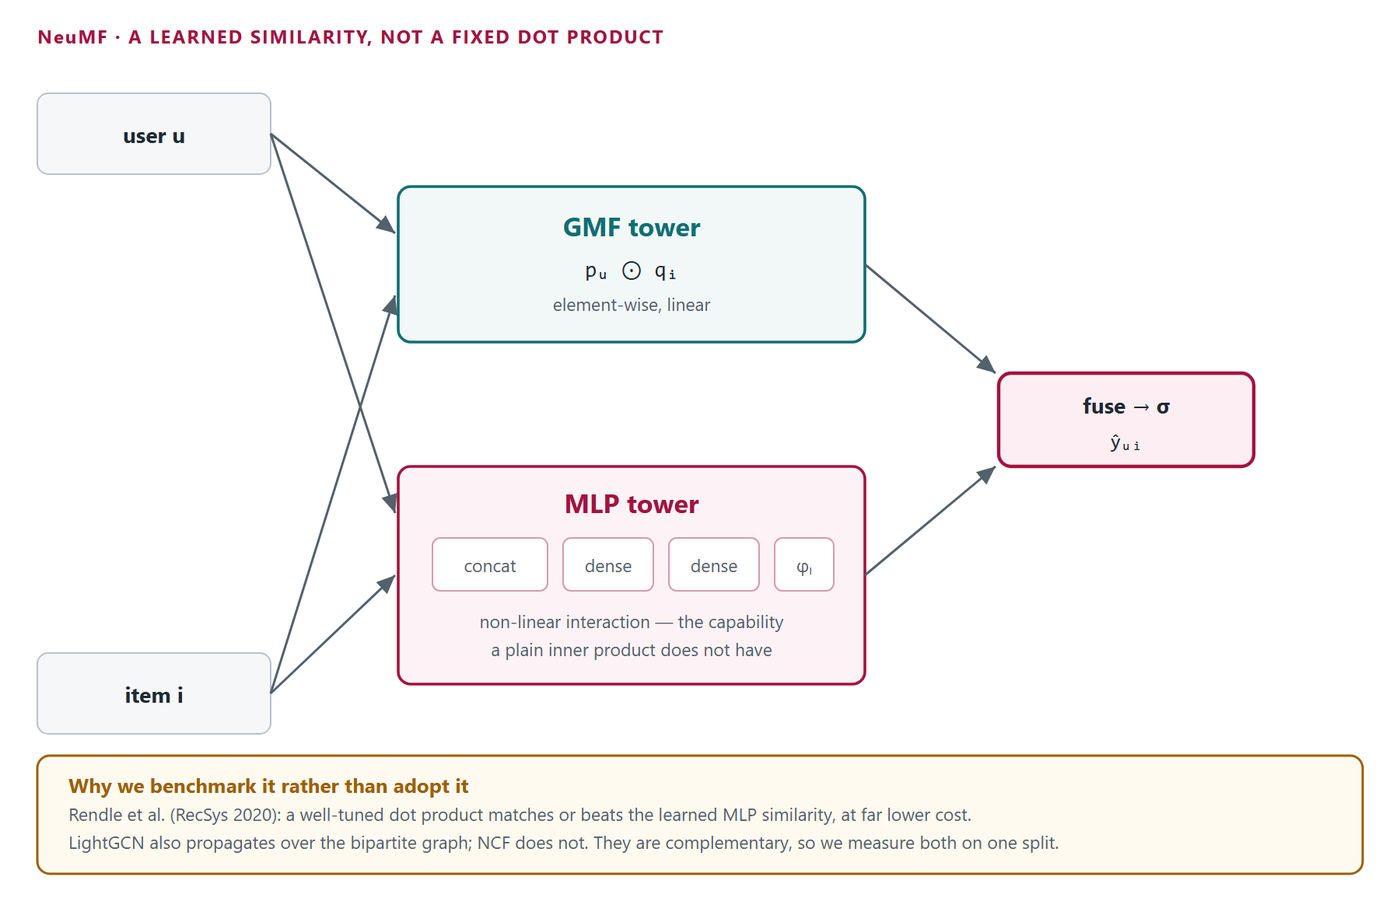
\includegraphics[width=\linewidth,height=4.9cm,keepaspectratio]{ncf}
\end{center}
\vspace{1mm}

\blk{Our position, and the plan}
\begin{tight}
  \item Rendle et al.\ (RecSys 2020) revisited this comparison and found a \textbf{well-tuned dot
        product matches or beats} the learned MLP, at far lower cost --- so we will run NeuMF as a
        \emph{measured baseline}, not adopt it as an assumed upgrade.
  \item The harness already runs three domains on fixed splits, so NeuMF slots in behind the same
        interface; then report popularity / LightGCN / NeuMF side by side.
\end{tight}
\end{columns}
\end{frame}

% ---------------------------------------------------------------------
\begin{frame}[shrink=15]{2. Model 3 --- Real-Time EMA User Vector}
\framesubtitle{Algorithm $\cdot$ equation $\cdot$ measured result}
\vspace{1mm}
\begin{columns}[T]
\column{0.515\textwidth}
\blk{Algorithm}
{\scriptsize A \textbf{signed, strength-scaled} exponential moving average in the same 384-d space
as the items. Not a plain average: a negative event pushes the user vector \emph{away} from the
item, and the step scales with how strong the event was.}
\vspace{1.5mm}

\blk{Equations, as implemented}
{\scriptsize
Event weight $w$: $+1.2$ complete, $+1.0$ like, $+0.6$ click, $+0.4$ view, $-1.0$ skip; a rating
$v$ maps to $(v-3)/2$. Then with $\alpha = 0.25$:
\[ d=\operatorname{sign}(w),\ \ s=\min(|w|,1),\ \ \eta=\operatorname{clip}(\alpha s,0,1) \]
\[ \mathbf{u}_{t+1} = \frac{(1-\eta)\mathbf{u}_t + \eta\,d\,\mathbf{e}_i}{\lVert\cdot\rVert_2},
   \ \ S_{\mathit{ema}} = \mathbf{u}_t^{\top}\mathbf{e}_i \]}

\column{0.46\textwidth}
\vspace{-3mm}
\begin{center}
  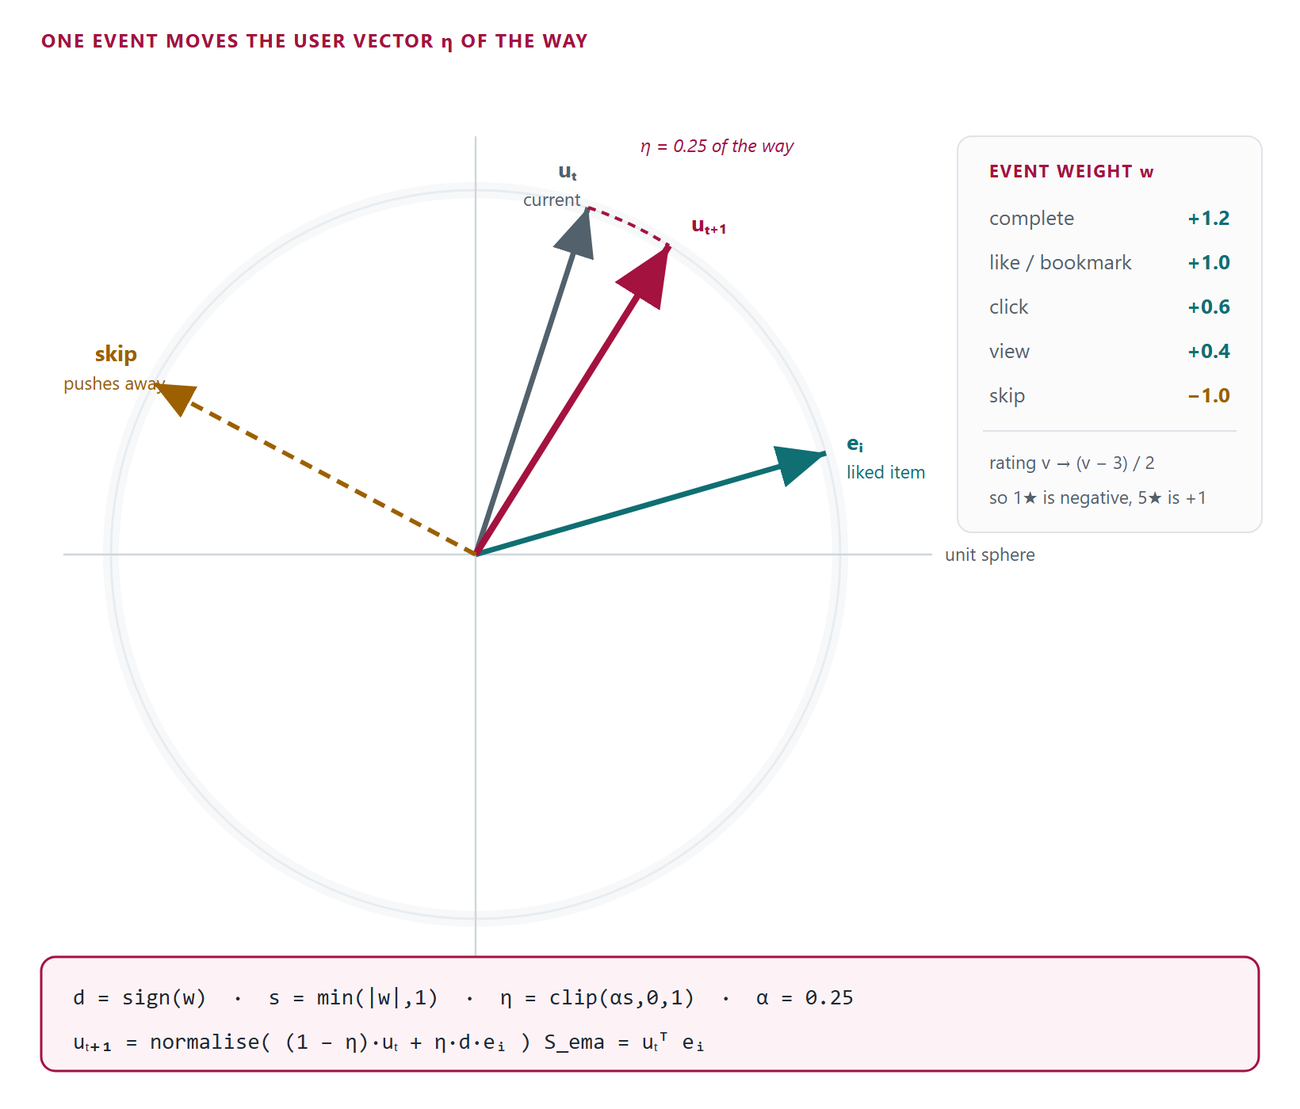
\includegraphics[width=\linewidth,height=5.5cm,keepaspectratio]{ema}
\end{center}
\vspace{1mm}

\blk{Measured}
\begin{tight}
  \item \textbf{39.0\,$\mu$s} per update, \textbf{16.7\,$\mu$s} per score (1{,}000 ops, 384-d).
  \item Against \textbf{hours} for a retrain --- five orders of magnitude. This is the "real-time"
        in the project title, as a number.
  \item \textbf{Limitation:} no session boundary or time decay, so one misclick persists.
\end{tight}
\end{columns}
\end{frame}

% ---------------------------------------------------------------------
\begin{frame}[shrink=15]{2. Model 4 --- Knowledge-Graph Overlap Head}
\framesubtitle{Algorithm $\cdot$ equation $\cdot$ measured result}
\vspace{1mm}
\begin{columns}[T]
\column{0.47\textwidth}
\blk{Algorithm and equation}
{\scriptsize A \textbf{zero-parameter set-overlap scorer} over shared entity namespaces. Nothing is
trained, so nothing drifts --- and it is defined precisely where the graph model is not. With
$T(i)$ the token set over \{title, description, creators, categories, type\}:
\[ S_{\mathit{kg}} = \min\!\left(1,\ \frac{|T(q)\cap T(i)|}{\max(3,|T(q)|)}\right) \]
The $\max(3,\cdot)$ floor stops a one-word query scoring 1.0 on one incidental match.}
\vspace{1.5mm}

\blk{Measured}
\begin{tight}
  \item Mean \textbf{KG@5 $=$ 0.892} over 8 scenarios; \textbf{0.667} on both named-entity queries,
        where dense retrieval smears.
  \item \textbf{Coverage 100\%} --- it reads metadata, not behaviour.
\end{tight}

\column{0.50\textwidth}
\vspace{-3mm}
\begin{center}
  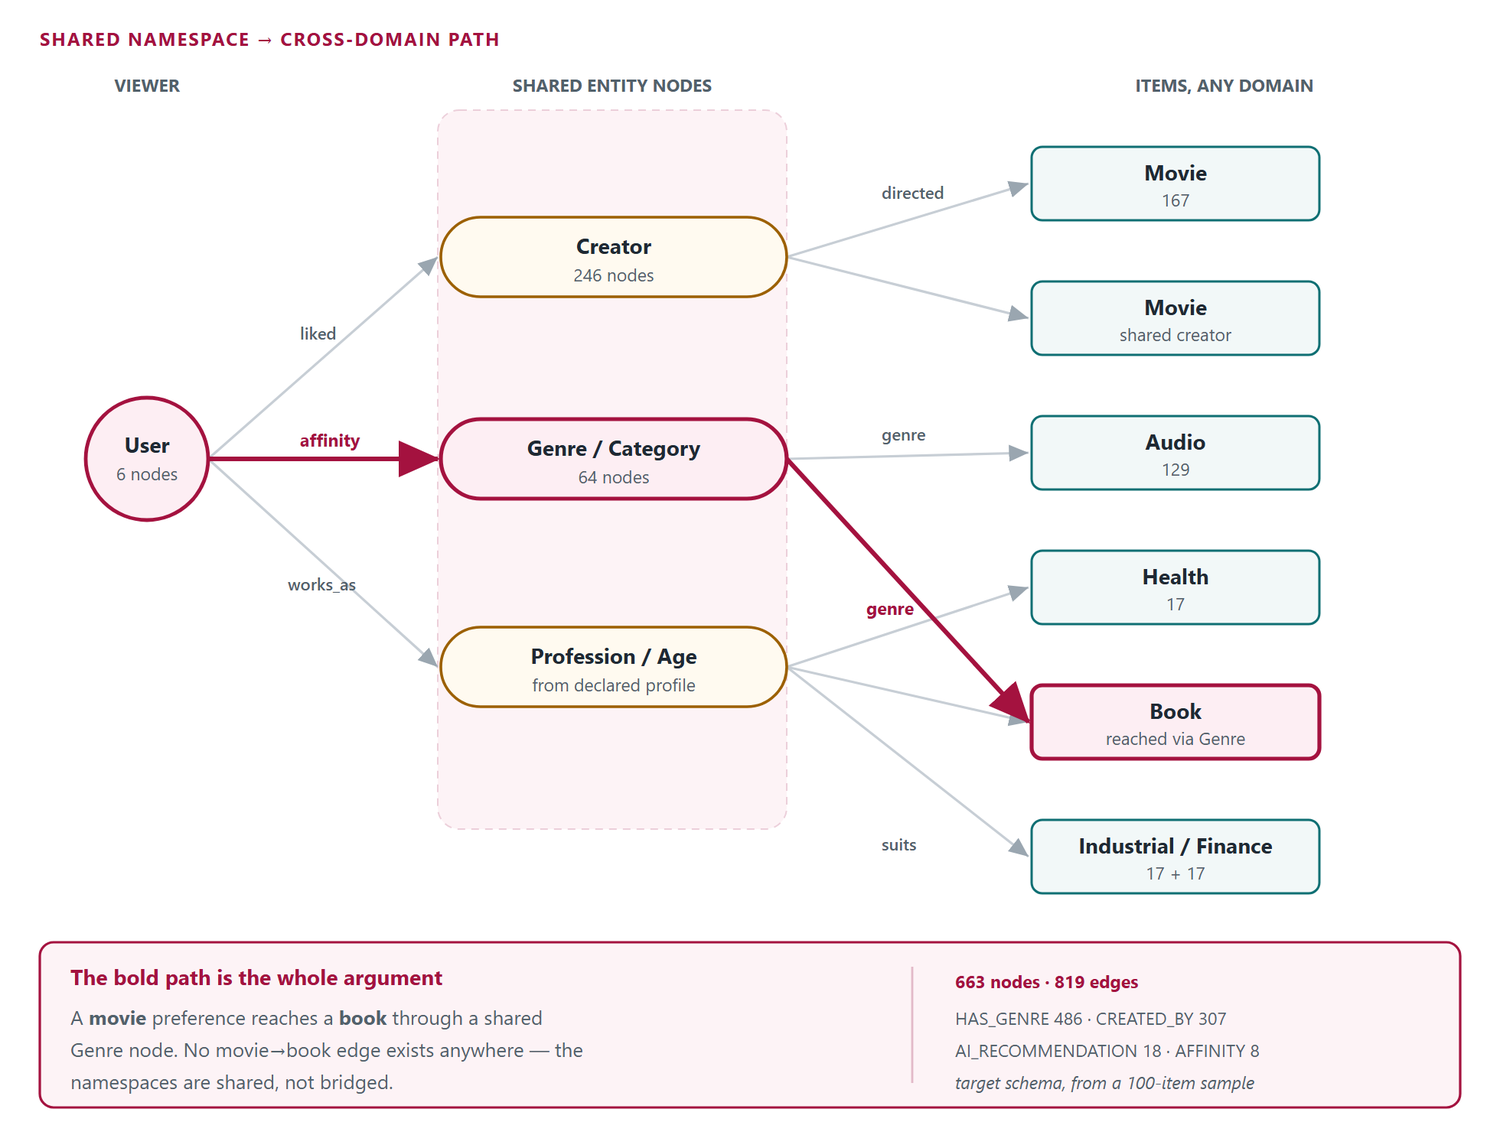
\includegraphics[width=\linewidth,height=5.7cm,keepaspectratio]{kg}
\end{center}
\vspace{1mm}

{\scriptsize\textcolor{amritaMaroon}{\textbf{Bold path:}} a \emph{movie} preference reaches a
\emph{book} through a shared Genre node --- no movie-to-book edge exists anywhere.}\\[1mm]
{\tiny\textbf{Scope.} At request time this is the overlap function above; the 663-node figure is the
\emph{target schema} from a 100-item example, not a runtime graph. Neo4j is Review 3.}
\end{columns}
\end{frame}

% ---------------------------------------------------------------------
\begin{frame}[shrink=15]{2. Model 5 --- Profile Head and the Eligibility Gate}
\framesubtitle{Algorithm $\cdot$ equation $\cdot$ measured result}
\vspace{1mm}
\begin{columns}[T]
\column{0.53\textwidth}
\blk{Profile head --- a score}
{\footnotesize A \textbf{weighted term matcher} against the declared profile; avoid-terms subtract
at nearly twice the weight of a positive match.
\[ S_{\mathit{profile}} = \operatorname{clip}\big(0.16|P\cap i| - 0.25|A\cap i| + 0.15\cdot\mathbf{1}[\tau_i \in \Pi]\big) \]}
\vspace{-3mm}
{\scriptsize $P$ = interests $\cup$ likes $\cup$ skills $\cup$ role $\cup$ age terms; \ $A$ = avoid
terms; \ $\Pi$ = preferred types; clipped to $[-1,1]$.}
\vspace{3mm}

\blk{Eligibility --- a predicate, not a score}
{\footnotesize
\[ \mathrm{elig}(i\,|\,c) = \mathbf{1}\big[a_{\mathit{eff}} \geq \mathrm{minage}(i)\big] \wedge \mathbf{1}\big[\tau_i \in \mathcal{T}(d)\big] \]
Compiled \emph{into} the Qdrant query, so an ineligible item is never retrieved, never scored, and
cannot be promoted back by any head.}
\vspace{2mm}

{\footnotesize\textbf{Fail-closed.} No age supplied caps at teen, not adult. Unknown metadata falls
back to the content-type default, never to unrestricted. Health and finance are \textbf{discovery
only, never advice}.}

\column{0.445\textwidth}
\vspace{-2mm}
\begin{center}
  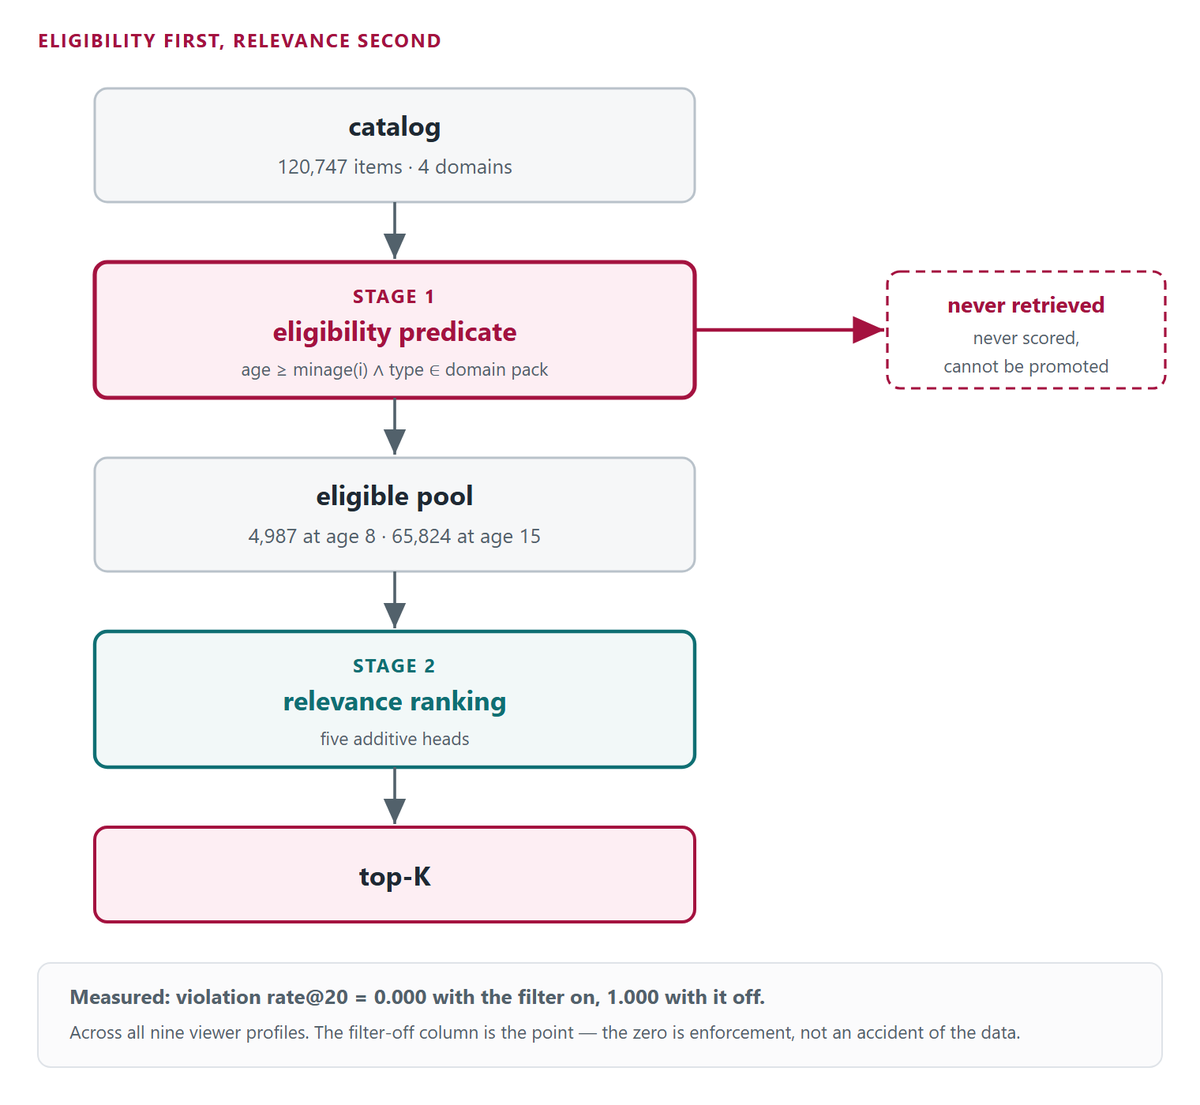
\includegraphics[width=\linewidth,height=5.9cm,keepaspectratio]{gate}
\end{center}
\vspace{2mm}
\blk{Measured}
\begin{tight}
  \item Mean \textbf{profile@5 $=$ 0.957}; \textbf{8 of 8} scenarios fully profile-positive.
  \item Violations \textbf{0.000} on, \textbf{1.000} off, across \textbf{9} viewer profiles.
\end{tight}
\end{columns}
\end{frame}
 from 2_presentation.tex
%
%  Every card carries the same four things in the same order:
%     ALGORITHM  --  what it is, by name
%     EQUATION   --  what the code computes
%     DIAGRAM    --  the mechanism, drawn
%     MEASURED   --  a number from this repository
%
%  HEIGHT BUDGET -- READ THIS BEFORE ADDING A LINE.
%  A 16:9 frame gives ~6.8cm of body once title, subtitle and footline
%  are paid for. That is about 20 lines at \scriptsize, 27 at \tiny.
%  A display equation \[..\] costs ~3 lines.
%
%  Every card carries [shrink=15]: beamer measures the frame and scales
%  it down ONLY if it would overflow, up to 15%. A frame that already
%  fits is untouched. This is a SAFETY NET, not a licence to overfill --
%  past 15% the content runs off the bottom edge silently, exactly as it
%  did before. If you add an equation, delete a bullet to pay for it.
%
%  Overleaf prints "Overfull \vbox" for any frame that needed shrinking;
%  that warning is the signal to cut a line, not to raise the 15%.
%
%  All figures measured from the repository, 14 Sep 2026.
% =====================================================================

% ---------------------------------------------------------------------
\begin{frame}[shrink=15]{2. Model Inventory --- Five Scoring Heads and One Gate}
\framesubtitle{Each is a different model class, defined where the others are not}
\vspace{1mm}
\begin{center}
{\scriptsize
\renewcommand{\arraystretch}{1.22}
\begin{tabular}{c L{2.5cm} L{3.9cm} c c c}
\toprule
\textbf{Head} & \textbf{Model class} & \textbf{What it computes} & \textbf{Range} & \textbf{Cov.} & \textbf{Wt.}\\
\midrule
$S_{\mathit{sem}}$     & Transformer encoder   & Cosine to a 384-d sentence embedding & $[-1,1]$ & \textbf{100\%} & $1.00$\\
$S_{\mathit{graph}}$   & Graph neural net (CF) & Inner product of LightGCN embeddings & $[-1,1]$ & \textcolor{amritaMaroon}{\textbf{0.20\%}} & $0.20$\\
$S_{\mathit{ema}}$     & Online moving average & Cosine to the live user vector       & $[-1,1]$ & \textbf{100\%} & $0.15$\\
$S_{\mathit{kg}}$      & Set overlap, 0 params & Query / entity token overlap         & $[0,1]$  & \textbf{100\%} & $0.08$\\
$S_{\mathit{profile}}$ & Weighted term matcher & Declared-profile alignment           & $[-1,1]$ & \textbf{100\%} & $0.10$\\
\midrule
\textit{gate} & \textit{Hard predicate} & \textit{May this viewer see this item at all?} & $\{0,1\}$ & \textbf{100\%} & \textit{---}\\
\bottomrule
\end{tabular}}
\end{center}
\vspace{1mm}
{\scriptsize
\[ S(q,u,i) = S_{\mathit{sem}} + 0.20\,S_{\mathit{graph}} + 0.15\,S_{\mathit{ema}} + 0.08\,S_{\mathit{kg}} + 0.10\,S_{\mathit{profile}} \]}
\vspace{-3mm}
{\scriptsize\textbf{Why coverage is the column that matters.} The graph head is our strongest signal
and is defined for \textbf{0.20\%} of the catalog; every other head is defined everywhere. That is
why the blend is additive with a dominant semantic term rather than a learned gate --- a missing
head must degrade the ranking, never break it.}
\end{frame}

% ---------------------------------------------------------------------
\begin{frame}[shrink=15]{2. Model 1 --- SBERT Semantic Encoder}
\framesubtitle{Algorithm $\cdot$ equation $\cdot$ measured result}
\vspace{1mm}
\begin{center}
  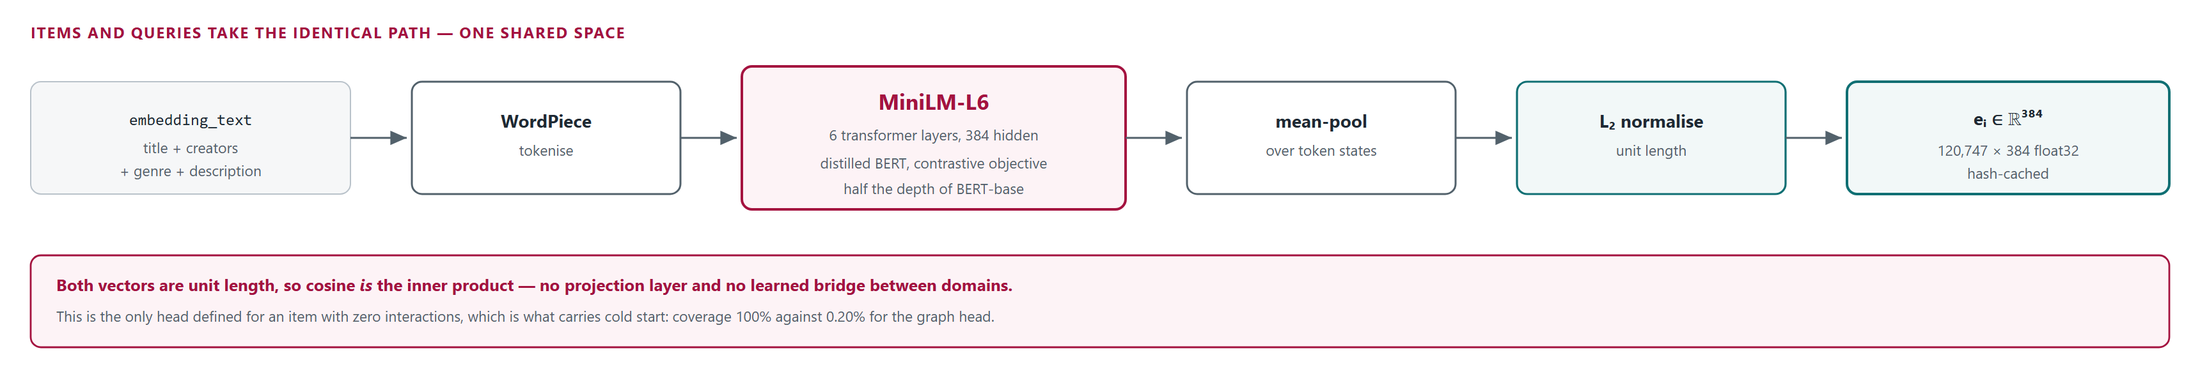
\includegraphics[width=\linewidth,height=3.4cm,keepaspectratio]{sbert}
\end{center}
\vspace{2mm}
\begin{columns}[T]
\column{0.485\textwidth}
\blk{Algorithm and equation}
{\scriptsize \texttt{all-MiniLM-L6-v2} --- a 6-layer distilled BERT, mean pooling over token states.
\[ \mathbf{e}_i = \frac{\mathrm{MeanPool}(\mathrm{MiniLM}(t_i))}{\lVert\cdot\rVert_2}, \quad
   S_{\mathit{sem}} = \mathbf{e}_i^{\top}\mathbf{q} \]
Both vectors are unit length, so cosine \emph{is} the inner product. The query takes the identical
path --- one shared space, no projection layer.}

\column{0.485\textwidth}
\blk{Measured}
\begin{tight}
  \item \textbf{120{,}747 $\times$ 384} float32; batch 256; hash-cached, so only changed rows
        re-encode.
  \item \textbf{Coverage 100\%} --- the only head defined at zero interactions, which is what
        carries cold start.
  \item 6 layers not 12, so the catalog encodes in one GPU pass and serving stays CPU-only.
\end{tight}
\end{columns}
\end{frame}

% ---------------------------------------------------------------------
\begin{frame}[shrink=15]{2. Model 2 --- LightGCN Graph Collaborative Filtering}
\framesubtitle{Algorithm $\cdot$ equation $\cdot$ measured result}
\vspace{1mm}
\begin{columns}[T]
\column{0.45\textwidth}
\blk{Algorithm}
{\scriptsize LightGCN (He et al., SIGIR 2020) --- a \emph{linear} convolution on the user--item
bipartite graph. Unlike NGCF there is \textbf{no feature transform and no nonlinearity}; the only
learned parameters are the layer-0 embeddings.}
\vspace{1.5mm}

\blk{Equations, as implemented}
{\scriptsize
With $\tilde{A} = D^{-1/2} A D^{-1/2}$, propagate and take the layer mean:
\[ \mathbf{E}^{(\ell)} = \tilde{A}\mathbf{E}^{(\ell-1)}, \quad
   \mathbf{E} = \tfrac{1}{L+1}\textstyle\sum_{\ell=0}^{L}\mathbf{E}^{(\ell)} \]
Score, and train by the BPR pairwise objective:
\[ \hat y_{ui} = \mathbf{e}_u^{\top}\mathbf{e}_i \]
\[ \mathcal{L} = -\!\sum \ln\sigma(\hat y_{ui}-\hat y_{uj}) + \lambda\lVert\mathbf{E}^{(0)}\rVert^2 \]}
\vspace{-1mm}
{\tiny\textbf{Config:} $d{=}64$, $L{=}3$, lr $10^{-3}$, decay $10^{-4}$, batch \textbf{4096},
60 epochs, seed 42, Kaggle T4.}

\column{0.52\textwidth}
\blk{Measured --- against a popularity control}
{\tiny
\renewcommand{\arraystretch}{1.15}
\begin{tabular}{L{1.4cm} l c c c c}
\toprule
\textbf{Domain} & \textbf{Model} & \textbf{R@20} & \textbf{N@20} & \textbf{MRR} & \textbf{Lift}\\
\midrule
Movies \& TV & LightGCN & \textbf{0.0288} & \textbf{0.0125} & \textbf{0.0080} & \\
             & popular  & 0.0182 & 0.0080 & 0.0052 & \textbf{1.59$\times$}\\
\midrule
Industrial   & LightGCN & \textbf{0.0326} & \textbf{0.0138} & \textbf{0.0087} & \\
             & popular  & 0.0264 & 0.0111 & 0.0070 & \textbf{1.24$\times$}\\
\midrule
Health       & LightGCN & 0.0121 & 0.0046 & 0.0025 & \\
             & popular  & \textbf{0.0221} & \textbf{0.0093} & \textbf{0.0059} & \textcolor{amritaMaroon}{\textbf{0.55$\times$}}\\
\bottomrule
\end{tabular}}\\[1.5mm]
{\tiny\textbf{Protocol.} Ratings $\geq 4$ as implicit positives; 10-core (Industrial keeps the
source 5-core floor); leave-last-out; 49{,}958 / 33{,}929 / 50{,}000 users evaluated.}\\[1.5mm]
{\tiny\textbf{$\mathtt{recall}=\mathtt{hit\_rate}$ is correct, not a bug:} leave-last-out gives one
relevant item, so Recall@$K \equiv$ HitRate@$K$. Check: $0.0288/20 = 0.00144$.}\\[1.5mm]
{\tiny\textcolor{amritaMaroon}{\textbf{Health regresses.}} BPR trains on the raw inner product, but
evaluation and serving both $L_2$-normalise and rank by cosine --- dividing by the \emph{item} norm
is not rank-preserving, and that norm carries the popularity prior.}
\end{columns}
\end{frame}

% ---------------------------------------------------------------------
%  PANEL RECOMMENDATION 1 -- NCF: position, architecture and plan
% ---------------------------------------------------------------------
\begin{frame}[shrink=15]{2. Panel Recommendation --- Neural Collaborative Filtering}
\framesubtitle{What NCF is, how it differs from LightGCN, and how we will test it}
\vspace{1mm}
\begin{columns}[T]
\column{0.475\textwidth}
\blk{What the panel asked for}
{\scriptsize NCF (He et al., WWW 2017) replaces the \emph{fixed} inner product with a \emph{learned}
similarity. NeuMF runs two towers and fuses them:
\[ \hat y^{\mathit{GMF}} = \mathbf{p}_u \odot \mathbf{q}_i, \quad
   \hat y^{\mathit{MLP}} = \phi_L(\cdots\phi_1([\mathbf{p}'_u \| \mathbf{q}'_i])) \]
\[ \hat y_{ui} = \sigma\big(\mathbf{h}^{\top}[\,\hat y^{\mathit{GMF}} \,\|\, \hat y^{\mathit{MLP}}\,]\big) \]
The MLP tower models \textbf{non-linear} interaction --- which our inner product cannot.}
\vspace{1.5mm}

\blk{How it differs from what we run}
\begin{tight}
  \item \textbf{LightGCN is graph-based:} it propagates over the bipartite graph, so a user is
        informed by items three hops away. \textbf{NCF has no graph} --- it learns a similarity on
        ids alone. They are complementary, not substitutes.
\end{tight}

\column{0.495\textwidth}
\vspace{-2mm}
\begin{center}
  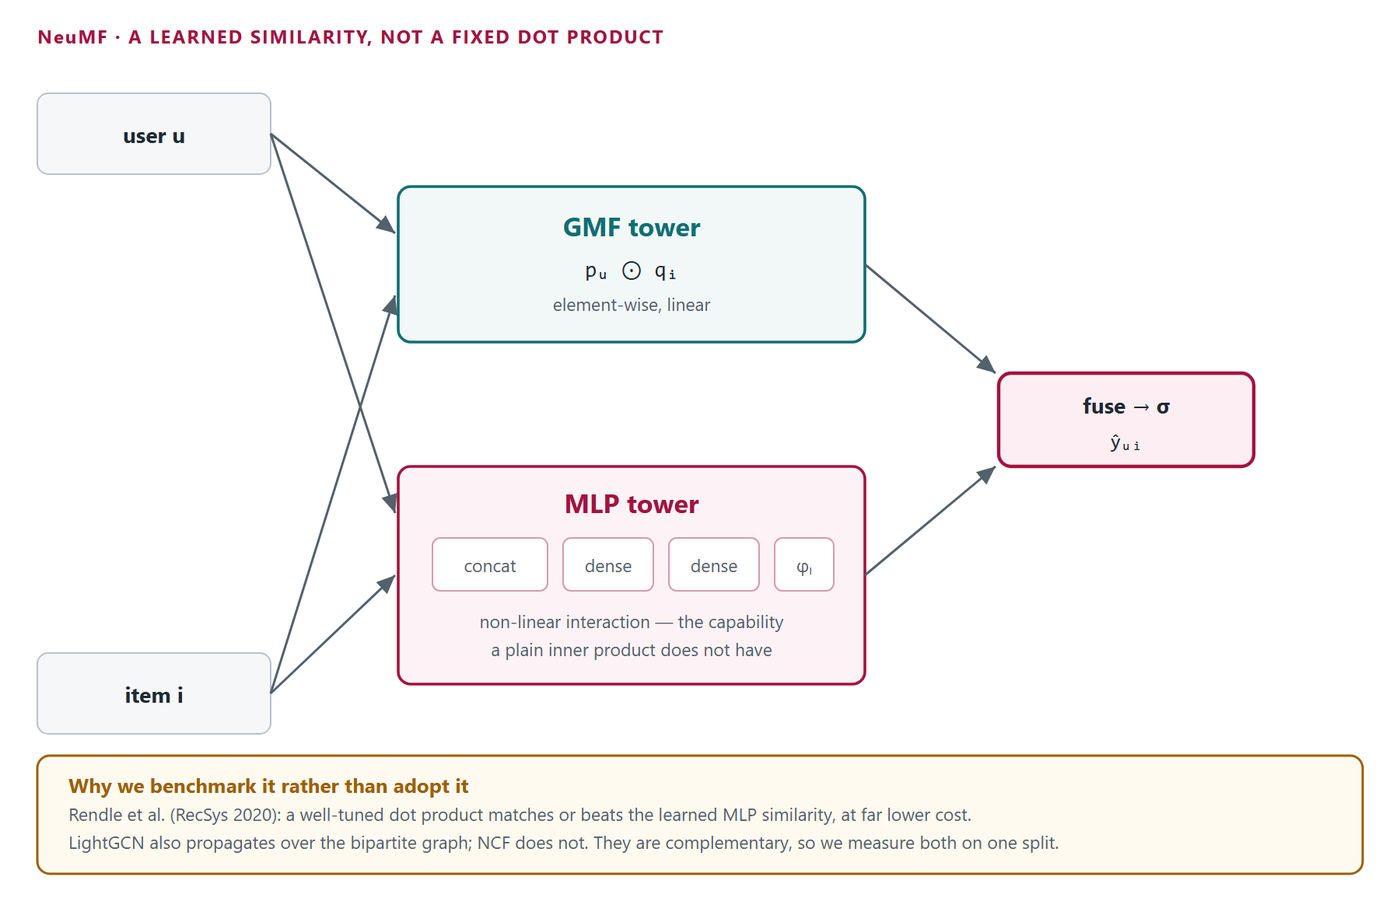
\includegraphics[width=\linewidth,height=4.9cm,keepaspectratio]{ncf}
\end{center}
\vspace{1mm}

\blk{Our position, and the plan}
\begin{tight}
  \item Rendle et al.\ (RecSys 2020) revisited this comparison and found a \textbf{well-tuned dot
        product matches or beats} the learned MLP, at far lower cost --- so we will run NeuMF as a
        \emph{measured baseline}, not adopt it as an assumed upgrade.
  \item The harness already runs three domains on fixed splits, so NeuMF slots in behind the same
        interface; then report popularity / LightGCN / NeuMF side by side.
\end{tight}
\end{columns}
\end{frame}

% ---------------------------------------------------------------------
\begin{frame}[shrink=15]{2. Model 3 --- Real-Time EMA User Vector}
\framesubtitle{Algorithm $\cdot$ equation $\cdot$ measured result}
\vspace{1mm}
\begin{columns}[T]
\column{0.515\textwidth}
\blk{Algorithm}
{\scriptsize A \textbf{signed, strength-scaled} exponential moving average in the same 384-d space
as the items. Not a plain average: a negative event pushes the user vector \emph{away} from the
item, and the step scales with how strong the event was.}
\vspace{1.5mm}

\blk{Equations, as implemented}
{\scriptsize
Event weight $w$: $+1.2$ complete, $+1.0$ like, $+0.6$ click, $+0.4$ view, $-1.0$ skip; a rating
$v$ maps to $(v-3)/2$. Then with $\alpha = 0.25$:
\[ d=\operatorname{sign}(w),\ \ s=\min(|w|,1),\ \ \eta=\operatorname{clip}(\alpha s,0,1) \]
\[ \mathbf{u}_{t+1} = \frac{(1-\eta)\mathbf{u}_t + \eta\,d\,\mathbf{e}_i}{\lVert\cdot\rVert_2},
   \ \ S_{\mathit{ema}} = \mathbf{u}_t^{\top}\mathbf{e}_i \]}

\column{0.46\textwidth}
\vspace{-3mm}
\begin{center}
  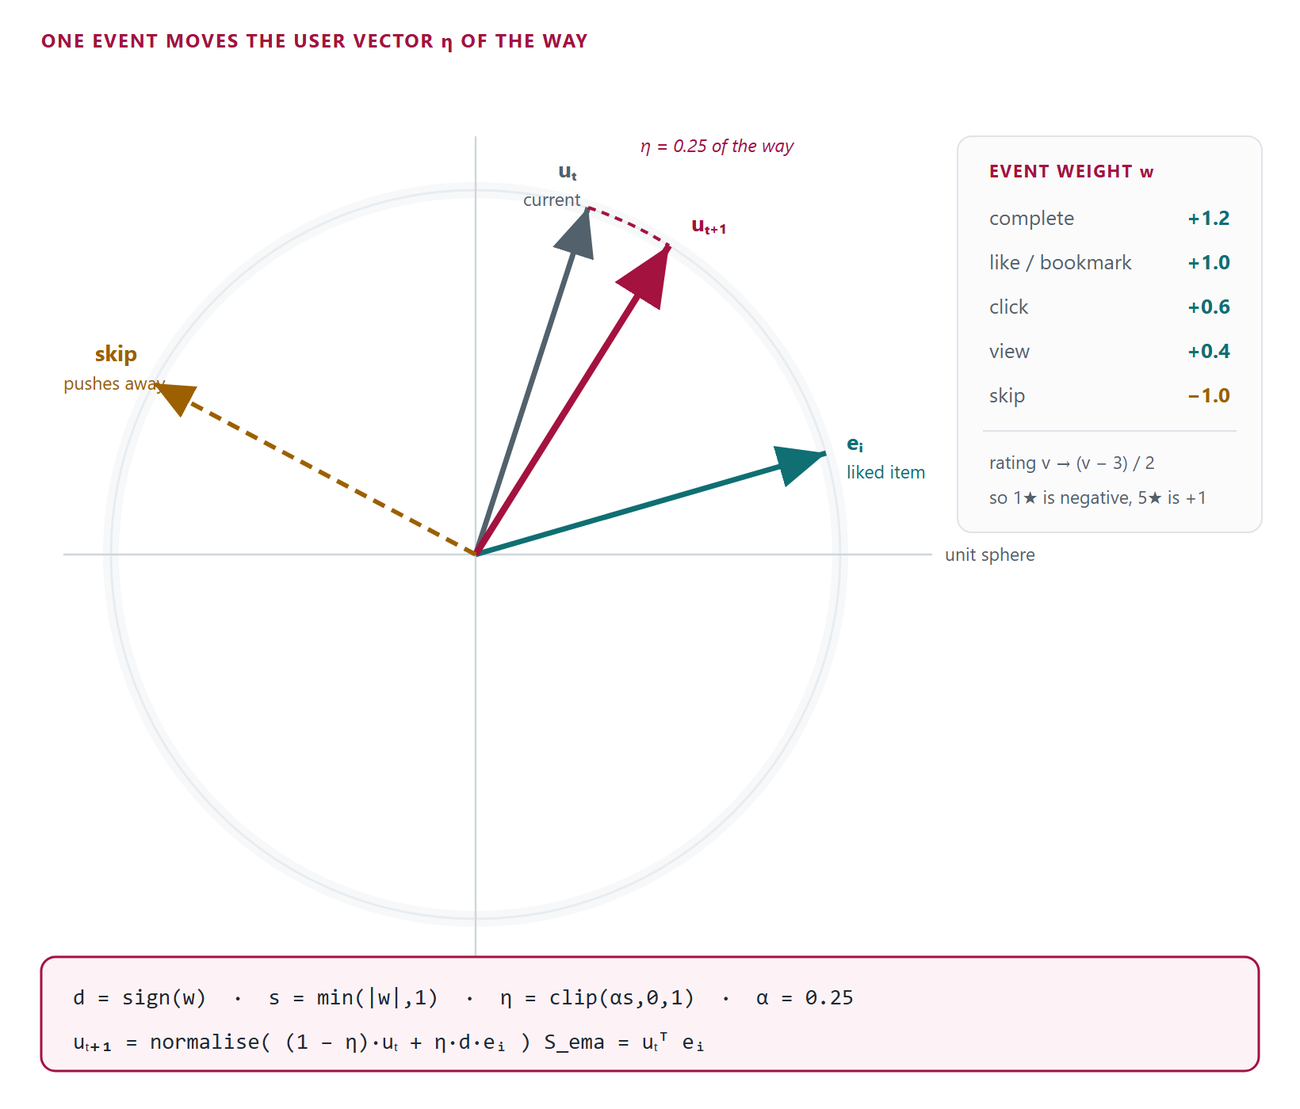
\includegraphics[width=\linewidth,height=5.5cm,keepaspectratio]{ema}
\end{center}
\vspace{1mm}

\blk{Measured}
\begin{tight}
  \item \textbf{39.0\,$\mu$s} per update, \textbf{16.7\,$\mu$s} per score (1{,}000 ops, 384-d).
  \item Against \textbf{hours} for a retrain --- five orders of magnitude. This is the "real-time"
        in the project title, as a number.
  \item \textbf{Limitation:} no session boundary or time decay, so one misclick persists.
\end{tight}
\end{columns}
\end{frame}

% ---------------------------------------------------------------------
\begin{frame}[shrink=15]{2. Model 4 --- Knowledge-Graph Overlap Head}
\framesubtitle{Algorithm $\cdot$ equation $\cdot$ measured result}
\vspace{1mm}
\begin{columns}[T]
\column{0.47\textwidth}
\blk{Algorithm and equation}
{\scriptsize A \textbf{zero-parameter set-overlap scorer} over shared entity namespaces. Nothing is
trained, so nothing drifts --- and it is defined precisely where the graph model is not. With
$T(i)$ the token set over \{title, description, creators, categories, type\}:
\[ S_{\mathit{kg}} = \min\!\left(1,\ \frac{|T(q)\cap T(i)|}{\max(3,|T(q)|)}\right) \]
The $\max(3,\cdot)$ floor stops a one-word query scoring 1.0 on one incidental match.}
\vspace{1.5mm}

\blk{Measured}
\begin{tight}
  \item Mean \textbf{KG@5 $=$ 0.892} over 8 scenarios; \textbf{0.667} on both named-entity queries,
        where dense retrieval smears.
  \item \textbf{Coverage 100\%} --- it reads metadata, not behaviour.
\end{tight}

\column{0.50\textwidth}
\vspace{-3mm}
\begin{center}
  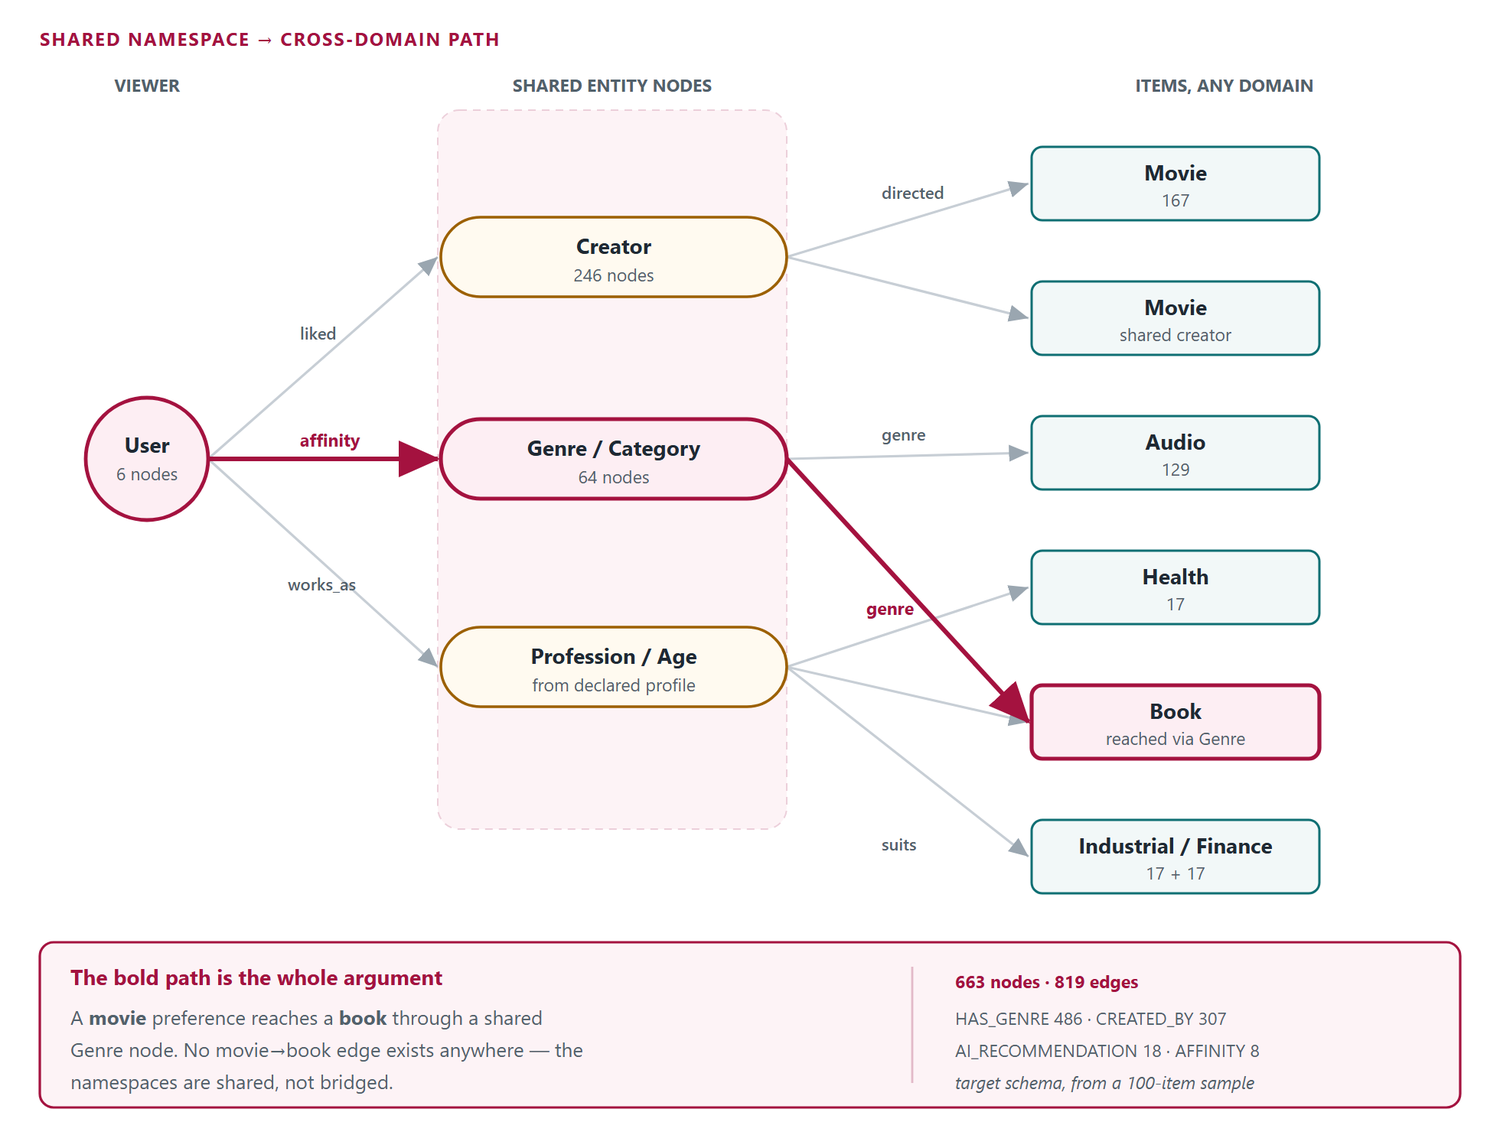
\includegraphics[width=\linewidth,height=5.7cm,keepaspectratio]{kg}
\end{center}
\vspace{1mm}

{\scriptsize\textcolor{amritaMaroon}{\textbf{Bold path:}} a \emph{movie} preference reaches a
\emph{book} through a shared Genre node --- no movie-to-book edge exists anywhere.}\\[1mm]
{\tiny\textbf{Scope.} At request time this is the overlap function above; the 663-node figure is the
\emph{target schema} from a 100-item example, not a runtime graph. Neo4j is Review 3.}
\end{columns}
\end{frame}

% ---------------------------------------------------------------------
\begin{frame}[shrink=15]{2. Model 5 --- Profile Head and the Eligibility Gate}
\framesubtitle{Algorithm $\cdot$ equation $\cdot$ measured result}
\vspace{1mm}
\begin{columns}[T]
\column{0.53\textwidth}
\blk{Profile head --- a score}
{\footnotesize A \textbf{weighted term matcher} against the declared profile; avoid-terms subtract
at nearly twice the weight of a positive match.
\[ S_{\mathit{profile}} = \operatorname{clip}\big(0.16|P\cap i| - 0.25|A\cap i| + 0.15\cdot\mathbf{1}[\tau_i \in \Pi]\big) \]}
\vspace{-3mm}
{\scriptsize $P$ = interests $\cup$ likes $\cup$ skills $\cup$ role $\cup$ age terms; \ $A$ = avoid
terms; \ $\Pi$ = preferred types; clipped to $[-1,1]$.}
\vspace{3mm}

\blk{Eligibility --- a predicate, not a score}
{\footnotesize
\[ \mathrm{elig}(i\,|\,c) = \mathbf{1}\big[a_{\mathit{eff}} \geq \mathrm{minage}(i)\big] \wedge \mathbf{1}\big[\tau_i \in \mathcal{T}(d)\big] \]
Compiled \emph{into} the Qdrant query, so an ineligible item is never retrieved, never scored, and
cannot be promoted back by any head.}
\vspace{2mm}

{\footnotesize\textbf{Fail-closed.} No age supplied caps at teen, not adult. Unknown metadata falls
back to the content-type default, never to unrestricted. Health and finance are \textbf{discovery
only, never advice}.}

\column{0.445\textwidth}
\vspace{-2mm}
\begin{center}
  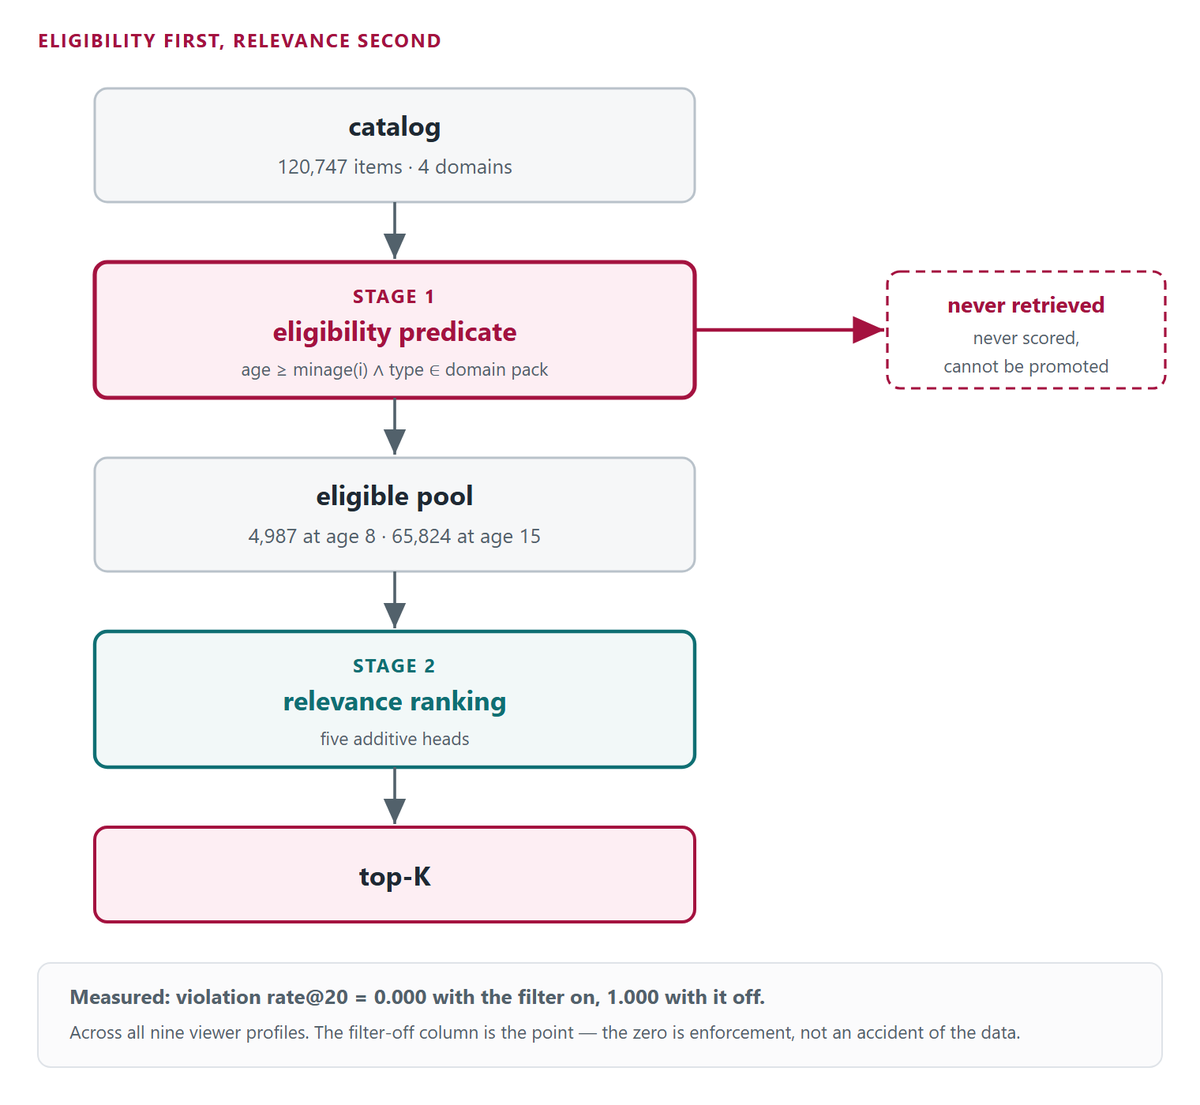
\includegraphics[width=\linewidth,height=5.9cm,keepaspectratio]{gate}
\end{center}
\vspace{2mm}
\blk{Measured}
\begin{tight}
  \item Mean \textbf{profile@5 $=$ 0.957}; \textbf{8 of 8} scenarios fully profile-positive.
  \item Violations \textbf{0.000} on, \textbf{1.000} off, across \textbf{9} viewer profiles.
\end{tight}
\end{columns}
\end{frame}


% =====================================================================
% ===== SPEAKER BLOCK: Aditya Vijay -- real-time adaptation
% =====================================================================
\section{Real-Time Adaptation}

% =====================================================================
% ===== SPEAKER BLOCK: Himaneesh Reddy J. -- constraints and audience
% =====================================================================
\section{Constraint \& Eligibility}

\begin{frame}[shrink=15]{2. Constraint \& Eligibility --- Domain Packs and Audience}
\framesubtitle{Eligibility first, relevance second}
\vspace{1mm}
\begin{columns}[T]
\column{0.515\textwidth}
\blk{The design argument, and how it changed}
\begin{tight}
  \item Safety began as a soft $-0.25$ demotion inside the reranker. That design \emph{fails}: a
        demoted item is still retrieved, so the graph, EMA or KG head can promote it back. A
        safety property must not be a tie-breaker.
  \item So safety moved out of scoring and into \textbf{eligibility}. The filter is compiled
        \emph{into the Qdrant query}, so an ineligible item is never retrieved, never scored, and
        cannot be promoted back by any head.
\end{tight}
\vspace{2mm}
\blk{Domain packs --- adding a vertical is a YAML entry}
\begin{tight}
  \item \textbf{Four domains:} Entertainment 77{,}644, Health 20{,}000, Industry 20{,}000,
        Finance 3{,}103.
  \item \textbf{Risk tiers:} 0 informational (97{,}644 items), 1 caution with advisory (23{,}103),
        2 professional, directory only.
  \item \textbf{Maturity ladder:} all\_ages 0, child 7, teen 13, young\_adult 16, adult 18,
        restricted 21.
\end{tight}

\column{0.455\textwidth}
\blk{Measured --- what it enforces, what it costs}
{\tiny
\renewcommand{\arraystretch}{1.38}
\begin{tabular}{p{1.95cm} c c c}
\toprule
\textbf{Viewer} & \textbf{Cover-} & \textbf{Viol.} & \textbf{Viol.}\\
                & \textbf{age}    & \textbf{ON}    & \textbf{OFF}\\
\midrule
Child (8)        & 4.1\%  & \textbf{0.000} & 1.000\\
Teen (15)        & 54.5\% & \textbf{0.000} & 1.000\\
Adult (25)       & 100\%  & \textbf{0.000} & 0.000\\
Adult, safe mode & 4.1\%  & \textbf{0.000} & 1.000\\
Age not supplied & 54.5\% & \textbf{0.000} & 1.000\\
\midrule
Entertainment    & 64.3\% & \textbf{0.000} & 1.000\\
Health           & 16.6\% & \textbf{0.000} & 0.100\\
Industry         & 16.6\% & \textbf{0.000} & 0.900\\
Finance          & 2.6\%  & \textbf{0.000} & 1.000\\
\bottomrule
\end{tabular}}\\[2.5mm]
{\tiny \textbf{Zero violations across all nine profiles}, over 120{,}747 items. The filter-off
column is the point: the zero is enforcement, not an accident of the data. We report the cost
too --- a child profile sees 4.1\% of the catalog.}
\end{columns}
\vspace{2mm}
\end{frame}

% ---------------------------------------------------------------------
\begin{frame}[shrink=15]{2. System in Action --- Audience Filtering}
\framesubtitle{The same query, the same profile, age 8 against age 25}
\vspace{0.5mm}
\begin{columns}[T]
\column{0.485\textwidth}
\begin{center}
\shot{age-child}{width=\linewidth,height=5.4cm,keepaspectratio}%
{Refine drawer open, age set to 8.}
\end{center}
\vspace{-1mm}
{\tiny\centering\textbf{Age 8} --- Strange World, Bubble, Ice Age, Spellbound\par}

\column{0.485\textwidth}
\begin{center}
\shot{age-adult}{width=\linewidth,height=5.4cm,keepaspectratio}%
{Refine drawer open, age set to 25.}
\end{center}
\vspace{-1mm}
{\tiny\centering\textbf{Age 25} --- Strange World, Johnny Test, Abenobashi, Fixed\par}
\end{columns}
\vspace{1.5mm}
\begin{columns}[T]
\column{0.485\textwidth}
\begin{itemize}\tiny\setlength{\itemsep}{2.5pt}
  \item Query \texttt{"fun animation adventure"} and profile are \textbf{identical} in both shots.
        Only the declared age differs, and the result set changes with it.
  \item The panel reports the ceiling back to the viewer: \textbf{SEES UP TO 7+} at age 8.
\end{itemize}

\column{0.485\textwidth}
\begin{itemize}\tiny\setlength{\itemsep}{2.5pt}
  \item No ranking code ran differently. The ineligible items were \textbf{never retrieved}, so no
        head could score or promote them --- which the panel itself states on screen.
  \item The two risk-tier-1 domains carry an advisory marker in the domain list.
\end{itemize}
\end{columns}
\end{frame}

% =====================================================================
% 3. TECHNICAL KNOWLEDGE  (5 Marks)
% =====================================================================
\section{Technical Knowledge}

\begin{frame}[shrink=15]{3. Technical Knowledge \& Engineering Decisions}
\framesubtitle{Rubric: Software Architecture, Implementation, Integration \& Tech Stack (5 Marks)}
\vspace{1mm}
\begin{columns}[T]
\column{0.485\textwidth}
\blk{Architecture and design patterns}
\begin{tight}
  \item \textbf{Layered} --- retrieval, storage, personalization and presentation are separately
        testable; the LightGCN artifact crosses a \emph{file} boundary, not a code boundary.
  \item \textbf{Registry} --- \texttt{domains.yaml} is read once into a \texttt{DomainRegistry}
        that drives the API, the filter and the UI. One source of truth for what a vertical is.
  \item \textbf{Repository} --- \texttt{MySQLStore} is the single SQL surface; no query text in a
        route handler.
  \item \textbf{Dependency injection} --- FastAPI \texttt{Depends} resolves the recommender, store
        and EMA singletons, so tests inject fakes without patching globals.
  \item \textbf{Lifespan singletons} --- heavy objects load once per worker, which fixed the
        storage-lock crash caused by reload's multi-process spawn.
\end{tight}

\column{0.485\textwidth}
\blk{Trade-offs we can defend}
\begin{tight}
  \item \textbf{BPR over MSE / BCE} --- feedback is implicit and positive-only, so there is no
        reliable negative label; ranking order is what we serve.
  \item \textbf{EMA over online gradients} --- one vector write per event, and item vectors stay
        untouched.
  \item \textbf{Config over code} --- a new vertical is a YAML entry. This is what makes the
        engine domain-agnostic rather than entertainment-shaped.
\end{tight}
\vspace{2mm}
\blk{Integrity, errors and testing}
\begin{tight}
  \item Foreign key pre-validated, so the API returns 400 rather than 500; idempotent upserts;
        composite index on the hot path.
  \item Graceful degradation --- a missing LightGCN artifact disables that head only; the other
        four still rank.
  \item \textbf{326} tests over 12 suites in \textbf{6.34\,s}; \texttt{oxlint} on the frontend.
\end{tight}
\end{columns}
\end{frame}

% ---------------------------------------------------------------------
\begin{frame}[shrink=15]{3. Is Each Module Justified?}
\framesubtitle{Why it matters $\cdot$ what breaks without it $\cdot$ is the current build defensible}
\vspace{1mm}
\begin{center}
{\tiny
\renewcommand{\arraystretch}{1.12}
\begin{tabular}{L{1.45cm} L{3.05cm} L{2.85cm} L{3.35cm}}
\toprule
\textbf{Module} & \textbf{Why it matters} & \textbf{What breaks without it} & \textbf{Current build defensible?}\\
\midrule
Data layer      & One schema over 9 sources makes cross-domain ranking possible.   & Every module needs per-source special cases.     & \textbf{Yes.} 120{,}747 rows, validated, 27 tests.\\
Domain registry & Adding a vertical becomes config, not code.                      & The engine stays entertainment-shaped.           & \textbf{Yes.} 4 packs live, driving real behaviour.\\
Embedding       & One space compares a film and a finance book directly.           & Cold-start items cannot be ranked at all.        & \textbf{Yes, with a caveat.} A tuned encoder is Review 3.\\
Retrieval       & Eligibility filters inside the ANN search, not after.            & Post-filtering lets ineligible items be scored.  & \textbf{Yes.} Hybrid lexical and vector.\\
Audience        & The safety property, as a hard predicate.                        & Age filtering degrades to a soft demotion.       & \textbf{Yes.} 0.000 violations over 9 profiles.\\
EMA             & Makes the "real-time adaptive" claim concrete.                   & Adaptation costs a retrain.                      & \textbf{Yes.} 39\,$\mu$s per event.\\
Graph CF        & Behaviour that text cannot express.                              & No collaborative signal at all.                  & \textbf{Partly.} Benchmarks real; served artifact is not.\\
Knowledge graph & Cross-domain bridge at zero parameters.                          & Named-entity queries smear.                      & \textbf{Yes, as scoped.} Graph DB is Review 3.\\
Persistence     & Interactions must survive a restart.                             & The feedback loop resets each restart.           & \textbf{Yes.} Validated, idempotent, indexed.\\
API + UI        & Every sub-score is returned, so results are explainable.         & The system becomes a black box.                  & \textbf{Yes.} 8 endpoints, 19 components.\\
\bottomrule
\end{tabular}}
\end{center}
\vspace{1mm}
{\tiny\textbf{Added in integration since the last review:} the eligibility filter compiled into the
search query $\cdot$ the domain registry driving API, filter and UI from one file $\cdot$ the matched
field surfaced end to end $\cdot$ risk-tier advisories from backend metadata $\cdot$ EMA writes inside
the interaction transaction.}
\end{frame}

% ---------------------------------------------------------------------
\begin{frame}[shrink=15]{3. Comparison with Existing Solutions}
\framesubtitle{Where this sits against production systems and published baselines}
\vspace{1mm}
\begin{center}
{\scriptsize
\renewcommand{\arraystretch}{1.25}
\begin{tabular}{L{3.1cm} c c c c}
\toprule
\textbf{System / approach} & \textbf{Cross-} & \textbf{Cold} & \textbf{Real-time} & \textbf{Eligibility}\\
                           & \textbf{domain} & \textbf{start}& \textbf{adaptation}& \textbf{layer}\\
\midrule
Netflix / Prime      & No     & Weak & Batch   & Ratings only\\
Spotify              & No     & Weak & Session & Explicit flag\\
Amazon item-to-item  & Partly & No   & Batch   & Category\\
LightFM / hybrid CF  & No     & Yes  & No      & No\\
Published LightGCN   & No     & No   & No      & No\\
\midrule
\textbf{This project} & \textbf{Yes, 4} & \textbf{Yes} & \textbf{Yes} & \textbf{Yes, hard}\\
\bottomrule
\end{tabular}}
\end{center}
\vspace{2mm}
\begin{columns}[T]
\column{0.485\textwidth}
\blk{Where ours is genuinely better}
\begin{itemize}\tiny\setlength{\itemsep}{2.5pt}
  \item \textbf{One query spans four unrelated domains.} A Netflix query cannot return a finance
        book; ours can, because namespaces are shared rather than bridged.
  \item \textbf{Eligibility is a hard pre-filter.} The systems above filter metadata \emph{after}
        retrieval; ours cannot retrieve an ineligible item at all.
  \item \textbf{Adding a vertical is a config change} --- no retraining, no new code path.
\end{itemize}

\column{0.485\textwidth}
\blk{Where we are behind}
\begin{itemize}\tiny\setlength{\itemsep}{2.5pt}
  \item \textbf{Data scale.} 914\,k interactions against their billions, so absolute recall is not
        comparable and we do not claim it is.
  \item \textbf{No online A/B evidence} --- every number here is offline or scenario-based.
  \item \textbf{The served LightGCN artifact is synthetic.} The benchmarks are real; the deployment
        is not yet.
\end{itemize}
\end{columns}
\vspace{1.5mm}
{\tiny\textbf{The fair claim} is not "better than Netflix". It is that the combination --- cross-domain
retrieval, cold-start coverage, real-time adaptation and hard eligibility in one serving path ---
is not something the systems above provide together.}
\end{frame}

% =====================================================================
% 4. TECHNICAL ENRICHMENT
% =====================================================================
\section{Technical Enrichment}

\begin{frame}{4. Technical Enrichment Activity Choices}
\framesubtitle{Professional Online Certification Details (Individual Mandatory: 10--20 Hours)}
\vspace{2mm}
\begin{center}
{\footnotesize
\renewcommand{\arraystretch}{1.40}
\begin{tabular}{|c|p{2.7cm}|p{4.3cm}|p{2.5cm}|c|}
\hline
\textbf{S.No} & \textbf{Student Name} & \textbf{Chosen MOOC / Course} & \textbf{Platform} & \textbf{Hours}\\
\hline
1 & Sanjay A. K.       & Recommender Systems: Evaluation and Metrics & Coursera (Minnesota) & 15 Hrs\\
\hline
2 & Eswara Raj M.      & Nearest Neighbor Collaborative Filtering    & Coursera (Minnesota) & 14 Hrs\\
\hline
3 & Aditya Vijay       & Databases and SQL for Data Science         & Coursera (IBM)       & 20 Hrs\\
\hline
4 & Himaneesh Reddy J. & Recommendation Systems on Google Cloud     & Google Cloud         & 16 Hrs\\
\hline
\end{tabular}}
\end{center}
\vspace{3mm}
\begin{itemize}\scriptsize\setlength{\itemsep}{4pt}
  \item \textbf{Project relevance:} the evaluation course supplies the Recall@K and NDCG@K protocol
  used on the metrics slide; neighbourhood collaborative filtering is the classical baseline
  LightGCN is measured against; SQL and indexing back the interaction store the EMA loop writes
  through; the Google Cloud course covers the same candidate-generation and reranking split our
  pipeline uses.
  \item \textbf{Requirement:} one approved 10--20 hour certification per student from a recognised
  platform relevant to the project. Certificates to be submitted at Review 3.
\end{itemize}
\end{frame}

% =====================================================================
% REFERENCES
% =====================================================================
\section{References}
\begin{frame}[allowframebreaks]{References}
    \scriptsize
    \nocite{*}
    \bibliographystyle{IEEEtran}
    \bibliography{ref}
\end{frame}

% =====================================================================
\begin{frame}
    \centering
    \vspace{0.8cm}
    {\Huge\textbf{\textcolor{amritaMaroon}{Thank You}}}\\[0.7cm]
    {\footnotesize\textcolor{amritaSlate}{Questions \& Panel Feedback}}
\end{frame}

% =====================================================================
% APPENDIX -- backup slides for Q&A, not presented
% =====================================================================
\section{Appendix}

\begin{frame}[shrink=15]{Appendix --- Scenario Evaluation Across All Four Domains}
\framesubtitle{Backup slide: measured end-to-end behaviour}
\vspace{1mm}
\begin{center}
{\scriptsize
\renewcommand{\arraystretch}{1.38}
\begin{tabular}{p{2.6cm} p{3.3cm} c c p{2.4cm}}
\toprule
\textbf{Scenario} & \textbf{Query} & \textbf{Hit@5} & \textbf{KG@5} & \textbf{Domains in top-10}\\
\midrule
Actor / director   & "James Cameron"               & 5/5 & 0.667 & book, movie\\
Singer / artist    & "Taylor Swift"                & 5/5 & 0.667 & music\\
Profession-aware   & "business analytics"          & --- & 1.000 & book, finance\\
Family-safe        & "fun animation adventure"     & --- & 1.000 & movie\\
Cross-media intent & "space adventure with aliens" & --- & 1.000 & book, movie\\
Health discovery   & "joint pain supplements"      & --- & 1.000 & health\\
Industrial lookup  & "protective safety gloves"    & --- & 0.900 & health, industrial\\
Finance literacy   & "personal budgeting"          & --- & 0.900 & finance\\
\bottomrule
\end{tabular}}
\end{center}
\vspace{2.5mm}
{\scriptsize\textbf{Reading this table.} \texttt{Hit@5} applies only to the two named-entity
queries --- for a topical query there is no single correct person to hit, so the cell is
deliberately blank rather than zero. \textbf{Four of eight} scenarios returned more than one media
type in the top-10, which is the cross-domain claim measured rather than asserted.}
\end{frame}

\begin{frame}[shrink=15]{Appendix --- Known Limitations and Next Steps}
\framesubtitle{Backup slide}
\vspace{1mm}
\begin{columns}[T]
\column{0.485\textwidth}
\blk{Open, in priority order}
\begin{enumerate}\scriptsize\setlength{\itemsep}{3.5pt}
  \item \textbf{The served LightGCN artifact is synthetic} --- 13 users, 347 items. The three
        domain benchmarks are real Kaggle runs; the artifact the API reranks with is not.
        Retraining at catalog scale is the highest-value next run.
  \item \textbf{The no-normalisation ablation is unrun.} It is the direct test of the
        health-regression hypothesis.
  \item \textbf{Finance has no benchmark row} --- Amazon has no finance category, so there is no
        interaction dataset for that vertical.
  \item \textbf{Maturity is heuristic} outside film, where TMDb certifications are fetched.
\end{enumerate}

\column{0.485\textwidth}
\blk{Planned for Review 3}
\begin{tight}
  \item Full-catalog LightGCN training, then the normalisation ablation on top of it.
  \item Neo4j-backed knowledge graph, so multi-hop paths are queried rather than approximated by
        token overlap.
  \item Per-session EMA vectors with a half-life decay term.
  \item Certified ratings extended from film to television and books.
  \item Docker Compose and CI; P95 latency under concurrent load.
\end{tight}
\vspace{2mm}
{\scriptsize The knowledge-graph and LightGCN caveats are one fact with two symptoms: the
visualizer's recommendation edges are built from that same synthetic artifact.}
\end{columns}
\end{frame}

\end{document}
